\section{Example}
\label{sec:example}

We will first explain the data that we use and how we use \ac{kde} to estimate the \ac{pdf}.
Next, we apply conditional sampling from the \ac{kde} according to \cref{alg:conditional simple,alg:conditional hard}.
Finally, we apply \cref{alg:constrained simple,alg:constrained hard} to sample from the \ac{kde} while the scenario parameters are subject to linear equality constraints.



\subsection{Data and \acp{kde}}
\label{sec:example data}

\cstarta We work with a data set obtained during an experiment in which 20 participants have driven a predefined route in The Netherlands.
The 50-kilometer route contained a variety of traffic elements, such as urban roads, motorways, junctions (with and without priority), pedestrian crossings, curvy road sections, traffic lights, speed bumps, etc.
The route took about 1 hour.
Because each participant drove the route thrice, the data set contains about 60 hours of driving.
Among other data, the speed of the participants was recorded.
As already done in \autocite{deGelder2017assessment, degelder2019completeness}, the speed was used to extract 2786 braking activities of the vehicle that is equipped with the sensors. \cenda
Each of the braking activities is described by $\dimension=3$ variables:
\begin{enumerate}
	\item the mean deceleration;
	\item the end speed; and
	\item the speed reduction.
\end{enumerate}

\cstarta To illustrate our method, we construct \iac{kde} of these parameters using the $\numberofsamples=2786$ data samples and sample a new set of parameters using the constructed \ac{kde}. \cenda
To apply \cref{alg:conditional simple,alg:constrained simple}, we employ \ac{kde} with the bandwidth matrix $\bandwidthmatrix=\bandwidth^2\identitymatrix{3}$. 
First, a diagonal bandwidth matrix is estimated using the plug-in selector of \textcite{wand1994multivariate}, as also explained in \autocite{duong2007ks}.
Then, the data points are scaled by the values at the diagonal, such that the bandwidth matrix $\bandwidthmatrix=\identitymatrix{3}$ can be used. 
The scaling is such that:
\begin{itemize}
	\item the first variable corresponds to the mean deceleration divided by $0.066$;
	\item the second variable corresponds to the end difference divided by $0.85$; and
	\item the third variable corresponds to the speed reduction divided by $0.55$.
\end{itemize}

To illustrate \cref{alg:conditional hard,alg:constrained hard}, we use a full bandwidth matrix $\bandwidthmatrix$. 
The bandwidth matrix is estimated using the plug-in selector of \textcite{wand1994multivariate}. 
The resulting bandwidth matrix is:
\begin{equation*}
	\bandwidthmatrix \approx
	\begin{bmatrix}
		0.0058 & -0.032 & 0.021 \\
		-0.032 & 0.92 & -0.23 \\
		0.021 & -0.23 & 0.40
	\end{bmatrix}.
\end{equation*}



\subsection{Sampling with part of $\variable$ fixed}

In this first example, we want to sample the speed difference, while the average deceleration equals $\SI{1}{\meter\per\second\squared}$ and the end speed equals $\SI{10}{\meter\per\second}$. 
Thus, we have two variables fixed ($\dimensionparta=2$) and one variable that is unconstrained ($\dimensionpartb=1$).

In \cref{fig:conditional simple,fig:conditional hard}, the result of \cref{alg:conditional simple,alg:conditional hard} is shown, respectively. 
In total, $10^6$ samples are generated and shown by the histogram (the bin width is \SI{0.2}{\meter\per\second}). 
Because the histograms follow the same pattern as the actual density of the speed difference according to the \ac{kde}, it illustrates that the provided algorithms correctly sample from the \ac{kde}. 

\begin{figure}
	\centering
	\resizebox{\columnwidth}{!}{%
		% Created by tikzDevice version 0.12.3 on 2021-02-14 20:34:46
% !TEX encoding = UTF-8 Unicode
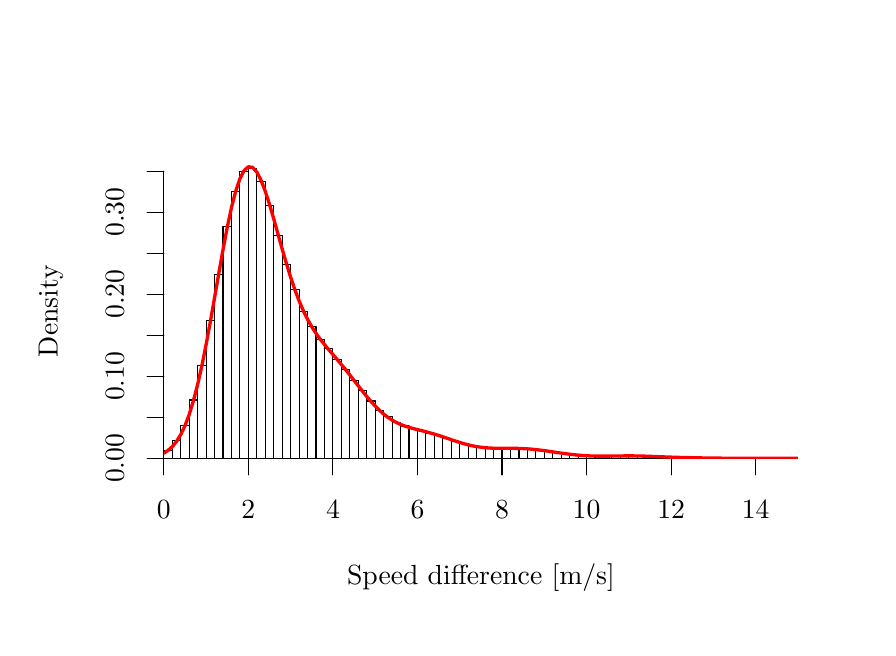
\begin{tikzpicture}[x=1pt,y=1pt]
\definecolor{fillColor}{RGB}{255,255,255}
\path[use as bounding box,fill=fillColor,fill opacity=0.00] (0,0) rectangle (303.53,216.81);
\begin{scope}
\path[clip] (  0.00,  0.00) rectangle (303.53,216.81);
\definecolor{drawColor}{RGB}{0,0,0}

\node[text=drawColor,anchor=base,inner sep=0pt, outer sep=0pt, scale=  1.00] at (163.77, 15.60) {Speed difference [m/s]};

\node[text=drawColor,rotate= 90.00,anchor=base,inner sep=0pt, outer sep=0pt, scale=  1.00] at ( 10.80,114.41) {Density};
\end{scope}
\begin{scope}
\path[clip] (  0.00,  0.00) rectangle (303.53,216.81);
\definecolor{drawColor}{RGB}{0,0,0}

\path[draw=drawColor,line width= 0.4pt,line join=round,line cap=round] ( 49.20, 61.20) -- (263.06, 61.20);

\path[draw=drawColor,line width= 0.4pt,line join=round,line cap=round] ( 49.20, 61.20) -- ( 49.20, 55.20);

\path[draw=drawColor,line width= 0.4pt,line join=round,line cap=round] ( 79.75, 61.20) -- ( 79.75, 55.20);

\path[draw=drawColor,line width= 0.4pt,line join=round,line cap=round] (110.30, 61.20) -- (110.30, 55.20);

\path[draw=drawColor,line width= 0.4pt,line join=round,line cap=round] (140.85, 61.20) -- (140.85, 55.20);

\path[draw=drawColor,line width= 0.4pt,line join=round,line cap=round] (171.40, 61.20) -- (171.40, 55.20);

\path[draw=drawColor,line width= 0.4pt,line join=round,line cap=round] (201.96, 61.20) -- (201.96, 55.20);

\path[draw=drawColor,line width= 0.4pt,line join=round,line cap=round] (232.51, 61.20) -- (232.51, 55.20);

\path[draw=drawColor,line width= 0.4pt,line join=round,line cap=round] (263.06, 61.20) -- (263.06, 55.20);

\node[text=drawColor,anchor=base,inner sep=0pt, outer sep=0pt, scale=  1.00] at ( 49.20, 39.60) {0};

\node[text=drawColor,anchor=base,inner sep=0pt, outer sep=0pt, scale=  1.00] at ( 79.75, 39.60) {2};

\node[text=drawColor,anchor=base,inner sep=0pt, outer sep=0pt, scale=  1.00] at (110.30, 39.60) {4};

\node[text=drawColor,anchor=base,inner sep=0pt, outer sep=0pt, scale=  1.00] at (140.85, 39.60) {6};

\node[text=drawColor,anchor=base,inner sep=0pt, outer sep=0pt, scale=  1.00] at (171.40, 39.60) {8};

\node[text=drawColor,anchor=base,inner sep=0pt, outer sep=0pt, scale=  1.00] at (201.96, 39.60) {10};

\node[text=drawColor,anchor=base,inner sep=0pt, outer sep=0pt, scale=  1.00] at (232.51, 39.60) {12};

\node[text=drawColor,anchor=base,inner sep=0pt, outer sep=0pt, scale=  1.00] at (263.06, 39.60) {14};

\path[draw=drawColor,line width= 0.4pt,line join=round,line cap=round] ( 49.20, 61.20) -- ( 49.20,164.97);

\path[draw=drawColor,line width= 0.4pt,line join=round,line cap=round] ( 49.20, 61.20) -- ( 43.20, 61.20);

\path[draw=drawColor,line width= 0.4pt,line join=round,line cap=round] ( 49.20, 76.02) -- ( 43.20, 76.02);

\path[draw=drawColor,line width= 0.4pt,line join=round,line cap=round] ( 49.20, 90.85) -- ( 43.20, 90.85);

\path[draw=drawColor,line width= 0.4pt,line join=round,line cap=round] ( 49.20,105.67) -- ( 43.20,105.67);

\path[draw=drawColor,line width= 0.4pt,line join=round,line cap=round] ( 49.20,120.50) -- ( 43.20,120.50);

\path[draw=drawColor,line width= 0.4pt,line join=round,line cap=round] ( 49.20,135.32) -- ( 43.20,135.32);

\path[draw=drawColor,line width= 0.4pt,line join=round,line cap=round] ( 49.20,150.14) -- ( 43.20,150.14);

\path[draw=drawColor,line width= 0.4pt,line join=round,line cap=round] ( 49.20,164.97) -- ( 43.20,164.97);

\node[text=drawColor,rotate= 90.00,anchor=base,inner sep=0pt, outer sep=0pt, scale=  1.00] at ( 34.80, 61.20) {0.00};

\node[text=drawColor,rotate= 90.00,anchor=base,inner sep=0pt, outer sep=0pt, scale=  1.00] at ( 34.80, 90.85) {0.10};

\node[text=drawColor,rotate= 90.00,anchor=base,inner sep=0pt, outer sep=0pt, scale=  1.00] at ( 34.80,120.50) {0.20};

\node[text=drawColor,rotate= 90.00,anchor=base,inner sep=0pt, outer sep=0pt, scale=  1.00] at ( 34.80,150.14) {0.30};
\end{scope}
\begin{scope}
\path[clip] ( 49.20, 61.20) rectangle (278.33,167.61);
\definecolor{drawColor}{RGB}{0,0,0}

\path[draw=drawColor,line width= 0.4pt,line join=round,line cap=round] ( -2.74, 61.20) rectangle (  0.32, 61.20);

\path[draw=drawColor,line width= 0.4pt,line join=round,line cap=round] (  0.32, 61.20) rectangle (  3.37, 61.20);

\path[draw=drawColor,line width= 0.4pt,line join=round,line cap=round] (  3.37, 61.20) rectangle (  6.43, 61.20);

\path[draw=drawColor,line width= 0.4pt,line join=round,line cap=round] (  6.43, 61.20) rectangle (  9.48, 61.20);

\path[draw=drawColor,line width= 0.4pt,line join=round,line cap=round] (  9.48, 61.20) rectangle ( 12.54, 61.20);

\path[draw=drawColor,line width= 0.4pt,line join=round,line cap=round] ( 12.54, 61.20) rectangle ( 15.59, 61.20);

\path[draw=drawColor,line width= 0.4pt,line join=round,line cap=round] ( 15.59, 61.20) rectangle ( 18.65, 61.20);

\path[draw=drawColor,line width= 0.4pt,line join=round,line cap=round] ( 18.65, 61.20) rectangle ( 21.70, 61.20);

\path[draw=drawColor,line width= 0.4pt,line join=round,line cap=round] ( 21.70, 61.20) rectangle ( 24.76, 61.20);

\path[draw=drawColor,line width= 0.4pt,line join=round,line cap=round] ( 24.76, 61.20) rectangle ( 27.81, 61.20);

\path[draw=drawColor,line width= 0.4pt,line join=round,line cap=round] ( 27.81, 61.20) rectangle ( 30.87, 61.20);

\path[draw=drawColor,line width= 0.4pt,line join=round,line cap=round] ( 30.87, 61.20) rectangle ( 33.92, 61.21);

\path[draw=drawColor,line width= 0.4pt,line join=round,line cap=round] ( 33.92, 61.20) rectangle ( 36.98, 61.21);

\path[draw=drawColor,line width= 0.4pt,line join=round,line cap=round] ( 36.98, 61.20) rectangle ( 40.03, 61.24);

\path[draw=drawColor,line width= 0.4pt,line join=round,line cap=round] ( 40.03, 61.20) rectangle ( 43.09, 61.38);

\path[draw=drawColor,line width= 0.4pt,line join=round,line cap=round] ( 43.09, 61.20) rectangle ( 46.14, 61.67);

\path[draw=drawColor,line width= 0.4pt,line join=round,line cap=round] ( 46.14, 61.20) rectangle ( 49.20, 62.43);

\path[draw=drawColor,line width= 0.4pt,line join=round,line cap=round] ( 49.20, 61.20) rectangle ( 52.26, 64.09);

\path[draw=drawColor,line width= 0.4pt,line join=round,line cap=round] ( 52.26, 61.20) rectangle ( 55.31, 67.48);

\path[draw=drawColor,line width= 0.4pt,line join=round,line cap=round] ( 55.31, 61.20) rectangle ( 58.37, 73.09);

\path[draw=drawColor,line width= 0.4pt,line join=round,line cap=round] ( 58.37, 61.20) rectangle ( 61.42, 82.26);

\path[draw=drawColor,line width= 0.4pt,line join=round,line cap=round] ( 61.42, 61.20) rectangle ( 64.48, 94.60);

\path[draw=drawColor,line width= 0.4pt,line join=round,line cap=round] ( 64.48, 61.20) rectangle ( 67.53,110.85);

\path[draw=drawColor,line width= 0.4pt,line join=round,line cap=round] ( 67.53, 61.20) rectangle ( 70.59,127.75);

\path[draw=drawColor,line width= 0.4pt,line join=round,line cap=round] ( 70.59, 61.20) rectangle ( 73.64,145.03);

\path[draw=drawColor,line width= 0.4pt,line join=round,line cap=round] ( 73.64, 61.20) rectangle ( 76.70,157.74);

\path[draw=drawColor,line width= 0.4pt,line join=round,line cap=round] ( 76.70, 61.20) rectangle ( 79.75,164.95);

\path[draw=drawColor,line width= 0.4pt,line join=round,line cap=round] ( 79.75, 61.20) rectangle ( 82.81,165.88);

\path[draw=drawColor,line width= 0.4pt,line join=round,line cap=round] ( 82.81, 61.20) rectangle ( 85.86,161.28);

\path[draw=drawColor,line width= 0.4pt,line join=round,line cap=round] ( 85.86, 61.20) rectangle ( 88.92,152.68);

\path[draw=drawColor,line width= 0.4pt,line join=round,line cap=round] ( 88.92, 61.20) rectangle ( 91.97,141.69);

\path[draw=drawColor,line width= 0.4pt,line join=round,line cap=round] ( 91.97, 61.20) rectangle ( 95.03,131.39);

\path[draw=drawColor,line width= 0.4pt,line join=round,line cap=round] ( 95.03, 61.20) rectangle ( 98.08,122.29);

\path[draw=drawColor,line width= 0.4pt,line join=round,line cap=round] ( 98.08, 61.20) rectangle (101.14,114.38);

\path[draw=drawColor,line width= 0.4pt,line join=round,line cap=round] (101.14, 61.20) rectangle (104.19,108.69);

\path[draw=drawColor,line width= 0.4pt,line join=round,line cap=round] (104.19, 61.20) rectangle (107.25,104.18);

\path[draw=drawColor,line width= 0.4pt,line join=round,line cap=round] (107.25, 61.20) rectangle (110.30,100.85);

\path[draw=drawColor,line width= 0.4pt,line join=round,line cap=round] (110.30, 61.20) rectangle (113.36, 96.80);

\path[draw=drawColor,line width= 0.4pt,line join=round,line cap=round] (113.36, 61.20) rectangle (116.41, 93.30);

\path[draw=drawColor,line width= 0.4pt,line join=round,line cap=round] (116.41, 61.20) rectangle (119.47, 89.43);

\path[draw=drawColor,line width= 0.4pt,line join=round,line cap=round] (119.47, 61.20) rectangle (122.52, 85.85);

\path[draw=drawColor,line width= 0.4pt,line join=round,line cap=round] (122.52, 61.20) rectangle (125.58, 81.92);

\path[draw=drawColor,line width= 0.4pt,line join=round,line cap=round] (125.58, 61.20) rectangle (128.63, 78.43);

\path[draw=drawColor,line width= 0.4pt,line join=round,line cap=round] (128.63, 61.20) rectangle (131.69, 76.20);

\path[draw=drawColor,line width= 0.4pt,line join=round,line cap=round] (131.69, 61.20) rectangle (134.74, 74.15);

\path[draw=drawColor,line width= 0.4pt,line join=round,line cap=round] (134.74, 61.20) rectangle (137.80, 72.88);

\path[draw=drawColor,line width= 0.4pt,line join=round,line cap=round] (137.80, 61.20) rectangle (140.85, 71.81);

\path[draw=drawColor,line width= 0.4pt,line join=round,line cap=round] (140.85, 61.20) rectangle (143.91, 71.15);

\path[draw=drawColor,line width= 0.4pt,line join=round,line cap=round] (143.91, 61.20) rectangle (146.96, 70.25);

\path[draw=drawColor,line width= 0.4pt,line join=round,line cap=round] (146.96, 61.20) rectangle (150.02, 69.32);

\path[draw=drawColor,line width= 0.4pt,line join=round,line cap=round] (150.02, 61.20) rectangle (153.07, 68.38);

\path[draw=drawColor,line width= 0.4pt,line join=round,line cap=round] (153.07, 61.20) rectangle (156.13, 67.38);

\path[draw=drawColor,line width= 0.4pt,line join=round,line cap=round] (156.13, 61.20) rectangle (159.18, 66.59);

\path[draw=drawColor,line width= 0.4pt,line join=round,line cap=round] (159.18, 61.20) rectangle (162.24, 65.73);

\path[draw=drawColor,line width= 0.4pt,line join=round,line cap=round] (162.24, 61.20) rectangle (165.29, 65.32);

\path[draw=drawColor,line width= 0.4pt,line join=round,line cap=round] (165.29, 61.20) rectangle (168.35, 64.99);

\path[draw=drawColor,line width= 0.4pt,line join=round,line cap=round] (168.35, 61.20) rectangle (171.40, 64.87);

\path[draw=drawColor,line width= 0.4pt,line join=round,line cap=round] (171.40, 61.20) rectangle (174.46, 64.71);

\path[draw=drawColor,line width= 0.4pt,line join=round,line cap=round] (174.46, 61.20) rectangle (177.52, 64.75);

\path[draw=drawColor,line width= 0.4pt,line join=round,line cap=round] (177.52, 61.20) rectangle (180.57, 64.66);

\path[draw=drawColor,line width= 0.4pt,line join=round,line cap=round] (180.57, 61.20) rectangle (183.63, 64.56);

\path[draw=drawColor,line width= 0.4pt,line join=round,line cap=round] (183.63, 61.20) rectangle (186.68, 64.14);

\path[draw=drawColor,line width= 0.4pt,line join=round,line cap=round] (186.68, 61.20) rectangle (189.74, 63.88);

\path[draw=drawColor,line width= 0.4pt,line join=round,line cap=round] (189.74, 61.20) rectangle (192.79, 63.36);

\path[draw=drawColor,line width= 0.4pt,line join=round,line cap=round] (192.79, 61.20) rectangle (195.85, 62.89);

\path[draw=drawColor,line width= 0.4pt,line join=round,line cap=round] (195.85, 61.20) rectangle (198.90, 62.51);

\path[draw=drawColor,line width= 0.4pt,line join=round,line cap=round] (198.90, 61.20) rectangle (201.96, 62.27);

\path[draw=drawColor,line width= 0.4pt,line join=round,line cap=round] (201.96, 61.20) rectangle (205.01, 62.11);

\path[draw=drawColor,line width= 0.4pt,line join=round,line cap=round] (205.01, 61.20) rectangle (208.07, 61.93);

\path[draw=drawColor,line width= 0.4pt,line join=round,line cap=round] (208.07, 61.20) rectangle (211.12, 61.95);

\path[draw=drawColor,line width= 0.4pt,line join=round,line cap=round] (211.12, 61.20) rectangle (214.18, 61.96);

\path[draw=drawColor,line width= 0.4pt,line join=round,line cap=round] (214.18, 61.20) rectangle (217.23, 62.09);

\path[draw=drawColor,line width= 0.4pt,line join=round,line cap=round] (217.23, 61.20) rectangle (220.29, 62.03);

\path[draw=drawColor,line width= 0.4pt,line join=round,line cap=round] (220.29, 61.20) rectangle (223.34, 62.05);

\path[draw=drawColor,line width= 0.4pt,line join=round,line cap=round] (223.34, 61.20) rectangle (226.40, 61.93);

\path[draw=drawColor,line width= 0.4pt,line join=round,line cap=round] (226.40, 61.20) rectangle (229.45, 61.80);

\path[draw=drawColor,line width= 0.4pt,line join=round,line cap=round] (229.45, 61.20) rectangle (232.51, 61.68);

\path[draw=drawColor,line width= 0.4pt,line join=round,line cap=round] (232.51, 61.20) rectangle (235.56, 61.60);

\path[draw=drawColor,line width= 0.4pt,line join=round,line cap=round] (235.56, 61.20) rectangle (238.62, 61.49);

\path[draw=drawColor,line width= 0.4pt,line join=round,line cap=round] (238.62, 61.20) rectangle (241.67, 61.40);

\path[draw=drawColor,line width= 0.4pt,line join=round,line cap=round] (241.67, 61.20) rectangle (244.73, 61.33);

\path[draw=drawColor,line width= 0.4pt,line join=round,line cap=round] (244.73, 61.20) rectangle (247.78, 61.30);

\path[draw=drawColor,line width= 0.4pt,line join=round,line cap=round] (247.78, 61.20) rectangle (250.84, 61.27);

\path[draw=drawColor,line width= 0.4pt,line join=round,line cap=round] (250.84, 61.20) rectangle (253.89, 61.25);

\path[draw=drawColor,line width= 0.4pt,line join=round,line cap=round] (253.89, 61.20) rectangle (256.95, 61.22);

\path[draw=drawColor,line width= 0.4pt,line join=round,line cap=round] (256.95, 61.20) rectangle (260.00, 61.21);

\path[draw=drawColor,line width= 0.4pt,line join=round,line cap=round] (260.00, 61.20) rectangle (263.06, 61.21);

\path[draw=drawColor,line width= 0.4pt,line join=round,line cap=round] (263.06, 61.20) rectangle (266.11, 61.20);

\path[draw=drawColor,line width= 0.4pt,line join=round,line cap=round] (266.11, 61.20) rectangle (269.17, 61.20);

\path[draw=drawColor,line width= 0.4pt,line join=round,line cap=round] (269.17, 61.20) rectangle (272.22, 61.20);

\path[draw=drawColor,line width= 0.4pt,line join=round,line cap=round] (272.22, 61.20) rectangle (275.28, 61.20);

\path[draw=drawColor,line width= 0.4pt,line join=round,line cap=round] (275.28, 61.20) rectangle (278.33, 61.20);

\path[draw=drawColor,line width= 0.4pt,line join=round,line cap=round] (278.33, 61.20) rectangle (281.39, 61.20);

\path[draw=drawColor,line width= 0.4pt,line join=round,line cap=round] (281.39, 61.20) rectangle (284.44, 61.20);

\path[draw=drawColor,line width= 0.4pt,line join=round,line cap=round] (284.44, 61.20) rectangle (287.50, 61.20);

\path[draw=drawColor,line width= 0.4pt,line join=round,line cap=round] (287.50, 61.20) rectangle (290.55, 61.20);

\path[draw=drawColor,line width= 0.4pt,line join=round,line cap=round] (290.55, 61.20) rectangle (293.61, 61.20);

\path[draw=drawColor,line width= 0.4pt,line join=round,line cap=round] (293.61, 61.20) rectangle (296.66, 61.20);

\path[draw=drawColor,line width= 0.4pt,line join=round,line cap=round] (296.66, 61.20) rectangle (299.72, 61.20);

\path[draw=drawColor,line width= 0.4pt,line join=round,line cap=round] (299.72, 61.20) rectangle (302.77, 61.20);

\path[draw=drawColor,line width= 0.4pt,line join=round,line cap=round] (302.77, 61.20) rectangle (305.83, 61.20);
\definecolor{drawColor}{RGB}{255,0,0}

\path[draw=drawColor,line width= 1.2pt,line join=round,line cap=round] (  0.00, 61.20) --
	(  0.32, 61.20) --
	(  1.85, 61.20) --
	(  3.37, 61.20) --
	(  4.90, 61.20) --
	(  6.43, 61.20) --
	(  7.96, 61.20) --
	(  9.48, 61.20) --
	( 11.01, 61.20) --
	( 12.54, 61.20) --
	( 14.07, 61.20) --
	( 15.59, 61.20) --
	( 17.12, 61.20) --
	( 18.65, 61.20) --
	( 20.18, 61.20) --
	( 21.70, 61.20) --
	( 23.23, 61.20) --
	( 24.76, 61.20) --
	( 26.29, 61.20) --
	( 27.81, 61.20) --
	( 29.34, 61.20) --
	( 30.87, 61.20) --
	( 32.40, 61.20) --
	( 33.92, 61.21) --
	( 35.45, 61.21) --
	( 36.98, 61.23) --
	( 38.51, 61.25) --
	( 40.03, 61.29) --
	( 41.56, 61.36) --
	( 43.09, 61.48) --
	( 44.62, 61.67) --
	( 46.14, 61.96) --
	( 47.67, 62.42) --
	( 49.20, 63.09) --
	( 50.73, 64.05) --
	( 52.26, 65.42) --
	( 53.78, 67.28) --
	( 55.31, 69.76) --
	( 56.84, 72.98) --
	( 58.37, 77.02) --
	( 59.89, 81.98) --
	( 61.42, 87.87) --
	( 62.95, 94.66) --
	( 64.48,102.28) --
	( 66.00,110.54) --
	( 67.53,119.22) --
	( 69.06,128.02) --
	( 70.59,136.61) --
	( 72.11,144.64) --
	( 73.64,151.78) --
	( 75.17,157.72) --
	( 76.70,162.25) --
	( 78.22,165.21) --
	( 79.75,166.56) --
	( 81.28,166.32) --
	( 82.81,164.63) --
	( 84.33,161.67) --
	( 85.86,157.68) --
	( 87.39,152.94) --
	( 88.92,147.71) --
	( 90.44,142.26) --
	( 91.97,136.81) --
	( 93.50,131.55) --
	( 95.03,126.62) --
	( 96.55,122.11) --
	( 98.08,118.08) --
	( 99.61,114.53) --
	(101.14,111.42) --
	(102.66,108.72) --
	(104.19,106.35) --
	(105.72,104.23) --
	(107.25,102.30) --
	(108.77,100.47) --
	(110.30, 98.69) --
	(111.83, 96.90) --
	(113.36, 95.08) --
	(114.89, 93.22) --
	(116.41, 91.30) --
	(117.94, 89.35) --
	(119.47, 87.39) --
	(121.00, 85.44) --
	(122.52, 83.55) --
	(124.05, 81.75) --
	(125.58, 80.08) --
	(127.11, 78.55) --
	(128.63, 77.18) --
	(130.16, 76.00) --
	(131.69, 74.99) --
	(133.22, 74.14) --
	(134.74, 73.44) --
	(136.27, 72.86) --
	(137.80, 72.37) --
	(139.33, 71.95) --
	(140.85, 71.56) --
	(142.38, 71.18) --
	(143.91, 70.80) --
	(145.44, 70.38) --
	(146.96, 69.94) --
	(148.49, 69.47) --
	(150.02, 68.97) --
	(151.55, 68.45) --
	(153.07, 67.93) --
	(154.60, 67.42) --
	(156.13, 66.93) --
	(157.66, 66.47) --
	(159.18, 66.07) --
	(160.71, 65.71) --
	(162.24, 65.42) --
	(163.77, 65.20) --
	(165.29, 65.03) --
	(166.82, 64.91) --
	(168.35, 64.85) --
	(169.88, 64.82) --
	(171.40, 64.81) --
	(172.93, 64.81) --
	(174.46, 64.81) --
	(175.99, 64.80) --
	(177.52, 64.77) --
	(179.04, 64.71) --
	(180.57, 64.62) --
	(182.10, 64.50) --
	(183.63, 64.35) --
	(185.15, 64.17) --
	(186.68, 63.97) --
	(188.21, 63.76) --
	(189.74, 63.53) --
	(191.26, 63.30) --
	(192.79, 63.08) --
	(194.32, 62.87) --
	(195.85, 62.68) --
	(197.37, 62.50) --
	(198.90, 62.35) --
	(200.43, 62.23) --
	(201.96, 62.13) --
	(203.48, 62.05) --
	(205.01, 62.01) --
	(206.54, 61.98) --
	(208.07, 61.98) --
	(209.59, 61.99) --
	(211.12, 62.01) --
	(212.65, 62.03) --
	(214.18, 62.05) --
	(215.70, 62.07) --
	(217.23, 62.07) --
	(218.76, 62.07) --
	(220.29, 62.05) --
	(221.81, 62.01) --
	(223.34, 61.97) --
	(224.87, 61.91) --
	(226.40, 61.86) --
	(227.92, 61.79) --
	(229.45, 61.73) --
	(230.98, 61.67) --
	(232.51, 61.62) --
	(234.03, 61.57) --
	(235.56, 61.52) --
	(237.09, 61.48) --
	(238.62, 61.44) --
	(240.14, 61.40) --
	(241.67, 61.37) --
	(243.20, 61.35) --
	(244.73, 61.32) --
	(246.26, 61.30) --
	(247.78, 61.28) --
	(249.31, 61.27) --
	(250.84, 61.25) --
	(252.37, 61.24) --
	(253.89, 61.23) --
	(255.42, 61.22) --
	(256.95, 61.22) --
	(258.48, 61.21) --
	(260.00, 61.21) --
	(261.53, 61.21) --
	(263.06, 61.20) --
	(264.59, 61.20) --
	(266.11, 61.20) --
	(267.64, 61.20) --
	(269.17, 61.20) --
	(270.70, 61.20) --
	(272.22, 61.20) --
	(273.75, 61.20) --
	(275.28, 61.20) --
	(276.81, 61.20) --
	(278.33, 61.20) --
	(279.86, 61.20) --
	(281.39, 61.20) --
	(282.92, 61.20) --
	(284.44, 61.20) --
	(285.97, 61.20) --
	(287.50, 61.20) --
	(289.03, 61.20) --
	(290.55, 61.20) --
	(292.08, 61.20) --
	(293.61, 61.20) --
	(295.14, 61.20) --
	(296.66, 61.20) --
	(298.19, 61.20) --
	(299.72, 61.20) --
	(301.25, 61.20) --
	(302.77, 61.20) --
	(303.53, 61.20);
\end{scope}
\end{tikzpicture}

	}
	\caption{The histogram shows the result of the conditional sampling according to \cref{alg:conditional simple}. The red line represents the true \ac{pdf}.}
	\label{fig:conditional simple}
\end{figure}

\begin{figure}
	\centering
	\resizebox{\columnwidth}{!}{%
		% Created by tikzDevice version 0.12.3 on 2021-01-24 20:23:36
% !TEX encoding = UTF-8 Unicode
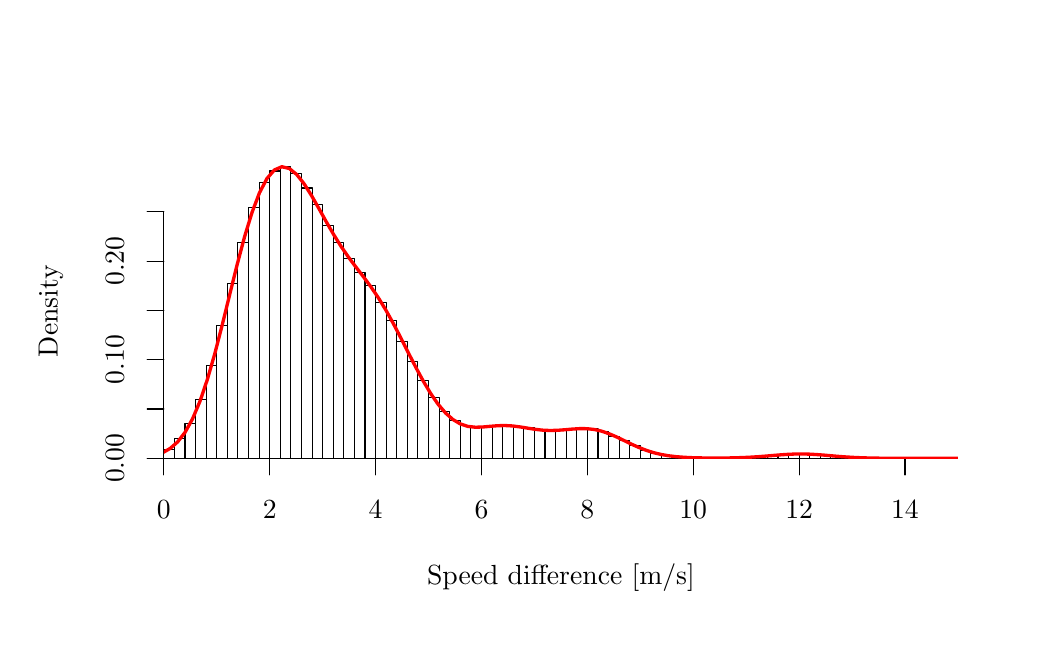
\begin{tikzpicture}[x=1pt,y=1pt]
\definecolor{fillColor}{RGB}{255,255,255}
\path[use as bounding box,fill=fillColor,fill opacity=0.00] (0,0) rectangle (361.35,216.81);
\begin{scope}
\path[clip] (  0.00,  0.00) rectangle (361.35,216.81);
\definecolor{drawColor}{RGB}{0,0,0}

\node[text=drawColor,anchor=base,inner sep=0pt, outer sep=0pt, scale=  1.00] at (192.68, 15.60) {Speed difference [m/s]};

\node[text=drawColor,rotate= 90.00,anchor=base,inner sep=0pt, outer sep=0pt, scale=  1.00] at ( 10.80,114.41) {Density};
\end{scope}
\begin{scope}
\path[clip] (  0.00,  0.00) rectangle (361.35,216.81);
\definecolor{drawColor}{RGB}{0,0,0}

\path[draw=drawColor,line width= 0.4pt,line join=round,line cap=round] ( 49.20, 61.20) -- (317.02, 61.20);

\path[draw=drawColor,line width= 0.4pt,line join=round,line cap=round] ( 49.20, 61.20) -- ( 49.20, 55.20);

\path[draw=drawColor,line width= 0.4pt,line join=round,line cap=round] ( 87.46, 61.20) -- ( 87.46, 55.20);

\path[draw=drawColor,line width= 0.4pt,line join=round,line cap=round] (125.72, 61.20) -- (125.72, 55.20);

\path[draw=drawColor,line width= 0.4pt,line join=round,line cap=round] (163.98, 61.20) -- (163.98, 55.20);

\path[draw=drawColor,line width= 0.4pt,line join=round,line cap=round] (202.24, 61.20) -- (202.24, 55.20);

\path[draw=drawColor,line width= 0.4pt,line join=round,line cap=round] (240.50, 61.20) -- (240.50, 55.20);

\path[draw=drawColor,line width= 0.4pt,line join=round,line cap=round] (278.76, 61.20) -- (278.76, 55.20);

\path[draw=drawColor,line width= 0.4pt,line join=round,line cap=round] (317.02, 61.20) -- (317.02, 55.20);

\node[text=drawColor,anchor=base,inner sep=0pt, outer sep=0pt, scale=  1.00] at ( 49.20, 39.60) {0};

\node[text=drawColor,anchor=base,inner sep=0pt, outer sep=0pt, scale=  1.00] at ( 87.46, 39.60) {2};

\node[text=drawColor,anchor=base,inner sep=0pt, outer sep=0pt, scale=  1.00] at (125.72, 39.60) {4};

\node[text=drawColor,anchor=base,inner sep=0pt, outer sep=0pt, scale=  1.00] at (163.98, 39.60) {6};

\node[text=drawColor,anchor=base,inner sep=0pt, outer sep=0pt, scale=  1.00] at (202.24, 39.60) {8};

\node[text=drawColor,anchor=base,inner sep=0pt, outer sep=0pt, scale=  1.00] at (240.50, 39.60) {10};

\node[text=drawColor,anchor=base,inner sep=0pt, outer sep=0pt, scale=  1.00] at (278.76, 39.60) {12};

\node[text=drawColor,anchor=base,inner sep=0pt, outer sep=0pt, scale=  1.00] at (317.02, 39.60) {14};

\path[draw=drawColor,line width= 0.4pt,line join=round,line cap=round] ( 49.20, 61.20) -- ( 49.20,150.23);

\path[draw=drawColor,line width= 0.4pt,line join=round,line cap=round] ( 49.20, 61.20) -- ( 43.20, 61.20);

\path[draw=drawColor,line width= 0.4pt,line join=round,line cap=round] ( 49.20, 79.01) -- ( 43.20, 79.01);

\path[draw=drawColor,line width= 0.4pt,line join=round,line cap=round] ( 49.20, 96.81) -- ( 43.20, 96.81);

\path[draw=drawColor,line width= 0.4pt,line join=round,line cap=round] ( 49.20,114.62) -- ( 43.20,114.62);

\path[draw=drawColor,line width= 0.4pt,line join=round,line cap=round] ( 49.20,132.42) -- ( 43.20,132.42);

\path[draw=drawColor,line width= 0.4pt,line join=round,line cap=round] ( 49.20,150.23) -- ( 43.20,150.23);

\node[text=drawColor,rotate= 90.00,anchor=base,inner sep=0pt, outer sep=0pt, scale=  1.00] at ( 34.80, 61.20) {0.00};

\node[text=drawColor,rotate= 90.00,anchor=base,inner sep=0pt, outer sep=0pt, scale=  1.00] at ( 34.80, 96.81) {0.10};

\node[text=drawColor,rotate= 90.00,anchor=base,inner sep=0pt, outer sep=0pt, scale=  1.00] at ( 34.80,132.42) {0.20};
\end{scope}
\begin{scope}
\path[clip] ( 49.20, 61.20) rectangle (336.15,167.61);
\definecolor{drawColor}{RGB}{0,0,0}

\path[draw=drawColor,line width= 0.4pt,line join=round,line cap=round] ( 18.59, 61.20) rectangle ( 22.42, 61.20);

\path[draw=drawColor,line width= 0.4pt,line join=round,line cap=round] ( 22.42, 61.20) rectangle ( 26.24, 61.20);

\path[draw=drawColor,line width= 0.4pt,line join=round,line cap=round] ( 26.24, 61.20) rectangle ( 30.07, 61.20);

\path[draw=drawColor,line width= 0.4pt,line join=round,line cap=round] ( 30.07, 61.20) rectangle ( 33.90, 61.22);

\path[draw=drawColor,line width= 0.4pt,line join=round,line cap=round] ( 33.90, 61.20) rectangle ( 37.72, 61.27);

\path[draw=drawColor,line width= 0.4pt,line join=round,line cap=round] ( 37.72, 61.20) rectangle ( 41.55, 61.42);

\path[draw=drawColor,line width= 0.4pt,line join=round,line cap=round] ( 41.55, 61.20) rectangle ( 45.37, 61.83);

\path[draw=drawColor,line width= 0.4pt,line join=round,line cap=round] ( 45.37, 61.20) rectangle ( 49.20, 62.68);

\path[draw=drawColor,line width= 0.4pt,line join=round,line cap=round] ( 49.20, 61.20) rectangle ( 53.03, 64.50);

\path[draw=drawColor,line width= 0.4pt,line join=round,line cap=round] ( 53.03, 61.20) rectangle ( 56.85, 68.20);

\path[draw=drawColor,line width= 0.4pt,line join=round,line cap=round] ( 56.85, 61.20) rectangle ( 60.68, 73.79);

\path[draw=drawColor,line width= 0.4pt,line join=round,line cap=round] ( 60.68, 61.20) rectangle ( 64.50, 82.61);

\path[draw=drawColor,line width= 0.4pt,line join=round,line cap=round] ( 64.50, 61.20) rectangle ( 68.33, 94.85);

\path[draw=drawColor,line width= 0.4pt,line join=round,line cap=round] ( 68.33, 61.20) rectangle ( 72.16,109.14);

\path[draw=drawColor,line width= 0.4pt,line join=round,line cap=round] ( 72.16, 61.20) rectangle ( 75.98,124.40);

\path[draw=drawColor,line width= 0.4pt,line join=round,line cap=round] ( 75.98, 61.20) rectangle ( 79.81,139.05);

\path[draw=drawColor,line width= 0.4pt,line join=round,line cap=round] ( 79.81, 61.20) rectangle ( 83.63,151.82);

\path[draw=drawColor,line width= 0.4pt,line join=round,line cap=round] ( 83.63, 61.20) rectangle ( 87.46,160.93);

\path[draw=drawColor,line width= 0.4pt,line join=round,line cap=round] ( 87.46, 61.20) rectangle ( 91.29,165.03);

\path[draw=drawColor,line width= 0.4pt,line join=round,line cap=round] ( 91.29, 61.20) rectangle ( 95.11,166.59);

\path[draw=drawColor,line width= 0.4pt,line join=round,line cap=round] ( 95.11, 61.20) rectangle ( 98.94,164.04);

\path[draw=drawColor,line width= 0.4pt,line join=round,line cap=round] ( 98.94, 61.20) rectangle (102.76,158.87);

\path[draw=drawColor,line width= 0.4pt,line join=round,line cap=round] (102.76, 61.20) rectangle (106.59,152.94);

\path[draw=drawColor,line width= 0.4pt,line join=round,line cap=round] (106.59, 61.20) rectangle (110.42,145.27);

\path[draw=drawColor,line width= 0.4pt,line join=round,line cap=round] (110.42, 61.20) rectangle (114.24,139.10);

\path[draw=drawColor,line width= 0.4pt,line join=round,line cap=round] (114.24, 61.20) rectangle (118.07,133.33);

\path[draw=drawColor,line width= 0.4pt,line join=round,line cap=round] (118.07, 61.20) rectangle (121.89,128.50);

\path[draw=drawColor,line width= 0.4pt,line join=round,line cap=round] (121.89, 61.20) rectangle (125.72,123.78);

\path[draw=drawColor,line width= 0.4pt,line join=round,line cap=round] (125.72, 61.20) rectangle (129.55,117.53);

\path[draw=drawColor,line width= 0.4pt,line join=round,line cap=round] (129.55, 61.20) rectangle (133.37,111.14);

\path[draw=drawColor,line width= 0.4pt,line join=round,line cap=round] (133.37, 61.20) rectangle (137.20,103.41);

\path[draw=drawColor,line width= 0.4pt,line join=round,line cap=round] (137.20, 61.20) rectangle (141.02, 96.18);

\path[draw=drawColor,line width= 0.4pt,line join=round,line cap=round] (141.02, 61.20) rectangle (144.85, 89.35);

\path[draw=drawColor,line width= 0.4pt,line join=round,line cap=round] (144.85, 61.20) rectangle (148.68, 83.11);

\path[draw=drawColor,line width= 0.4pt,line join=round,line cap=round] (148.68, 61.20) rectangle (152.50, 78.09);

\path[draw=drawColor,line width= 0.4pt,line join=round,line cap=round] (152.50, 61.20) rectangle (156.33, 74.80);

\path[draw=drawColor,line width= 0.4pt,line join=round,line cap=round] (156.33, 61.20) rectangle (160.15, 73.11);

\path[draw=drawColor,line width= 0.4pt,line join=round,line cap=round] (160.15, 61.20) rectangle (163.98, 72.71);

\path[draw=drawColor,line width= 0.4pt,line join=round,line cap=round] (163.98, 61.20) rectangle (167.81, 72.71);

\path[draw=drawColor,line width= 0.4pt,line join=round,line cap=round] (167.81, 61.20) rectangle (171.63, 73.15);

\path[draw=drawColor,line width= 0.4pt,line join=round,line cap=round] (171.63, 61.20) rectangle (175.46, 73.04);

\path[draw=drawColor,line width= 0.4pt,line join=round,line cap=round] (175.46, 61.20) rectangle (179.28, 72.54);

\path[draw=drawColor,line width= 0.4pt,line join=round,line cap=round] (179.28, 61.20) rectangle (183.11, 72.20);

\path[draw=drawColor,line width= 0.4pt,line join=round,line cap=round] (183.11, 61.20) rectangle (186.94, 71.35);

\path[draw=drawColor,line width= 0.4pt,line join=round,line cap=round] (186.94, 61.20) rectangle (190.76, 71.37);

\path[draw=drawColor,line width= 0.4pt,line join=round,line cap=round] (190.76, 61.20) rectangle (194.59, 71.51);

\path[draw=drawColor,line width= 0.4pt,line join=round,line cap=round] (194.59, 61.20) rectangle (198.41, 71.71);

\path[draw=drawColor,line width= 0.4pt,line join=round,line cap=round] (198.41, 61.20) rectangle (202.24, 71.87);

\path[draw=drawColor,line width= 0.4pt,line join=round,line cap=round] (202.24, 61.20) rectangle (206.07, 71.77);

\path[draw=drawColor,line width= 0.4pt,line join=round,line cap=round] (206.07, 61.20) rectangle (209.89, 70.85);

\path[draw=drawColor,line width= 0.4pt,line join=round,line cap=round] (209.89, 61.20) rectangle (213.72, 69.18);

\path[draw=drawColor,line width= 0.4pt,line join=round,line cap=round] (213.72, 61.20) rectangle (217.54, 67.48);

\path[draw=drawColor,line width= 0.4pt,line join=round,line cap=round] (217.54, 61.20) rectangle (221.37, 65.73);

\path[draw=drawColor,line width= 0.4pt,line join=round,line cap=round] (221.37, 61.20) rectangle (225.20, 64.18);

\path[draw=drawColor,line width= 0.4pt,line join=round,line cap=round] (225.20, 61.20) rectangle (229.02, 62.97);

\path[draw=drawColor,line width= 0.4pt,line join=round,line cap=round] (229.02, 61.20) rectangle (232.85, 62.23);

\path[draw=drawColor,line width= 0.4pt,line join=round,line cap=round] (232.85, 61.20) rectangle (236.67, 61.77);

\path[draw=drawColor,line width= 0.4pt,line join=round,line cap=round] (236.67, 61.20) rectangle (240.50, 61.51);

\path[draw=drawColor,line width= 0.4pt,line join=round,line cap=round] (240.50, 61.20) rectangle (244.33, 61.37);

\path[draw=drawColor,line width= 0.4pt,line join=round,line cap=round] (244.33, 61.20) rectangle (248.15, 61.29);

\path[draw=drawColor,line width= 0.4pt,line join=round,line cap=round] (248.15, 61.20) rectangle (251.98, 61.33);

\path[draw=drawColor,line width= 0.4pt,line join=round,line cap=round] (251.98, 61.20) rectangle (255.80, 61.36);

\path[draw=drawColor,line width= 0.4pt,line join=round,line cap=round] (255.80, 61.20) rectangle (259.63, 61.43);

\path[draw=drawColor,line width= 0.4pt,line join=round,line cap=round] (259.63, 61.20) rectangle (263.46, 61.62);

\path[draw=drawColor,line width= 0.4pt,line join=round,line cap=round] (263.46, 61.20) rectangle (267.28, 61.88);

\path[draw=drawColor,line width= 0.4pt,line join=round,line cap=round] (267.28, 61.20) rectangle (271.11, 62.23);

\path[draw=drawColor,line width= 0.4pt,line join=round,line cap=round] (271.11, 61.20) rectangle (274.93, 62.57);

\path[draw=drawColor,line width= 0.4pt,line join=round,line cap=round] (274.93, 61.20) rectangle (278.76, 62.76);

\path[draw=drawColor,line width= 0.4pt,line join=round,line cap=round] (278.76, 61.20) rectangle (282.59, 62.73);

\path[draw=drawColor,line width= 0.4pt,line join=round,line cap=round] (282.59, 61.20) rectangle (286.41, 62.59);

\path[draw=drawColor,line width= 0.4pt,line join=round,line cap=round] (286.41, 61.20) rectangle (290.24, 62.26);

\path[draw=drawColor,line width= 0.4pt,line join=round,line cap=round] (290.24, 61.20) rectangle (294.06, 61.96);

\path[draw=drawColor,line width= 0.4pt,line join=round,line cap=round] (294.06, 61.20) rectangle (297.89, 61.71);

\path[draw=drawColor,line width= 0.4pt,line join=round,line cap=round] (297.89, 61.20) rectangle (301.72, 61.48);

\path[draw=drawColor,line width= 0.4pt,line join=round,line cap=round] (301.72, 61.20) rectangle (305.54, 61.33);

\path[draw=drawColor,line width= 0.4pt,line join=round,line cap=round] (305.54, 61.20) rectangle (309.37, 61.25);

\path[draw=drawColor,line width= 0.4pt,line join=round,line cap=round] (309.37, 61.20) rectangle (313.19, 61.23);

\path[draw=drawColor,line width= 0.4pt,line join=round,line cap=round] (313.19, 61.20) rectangle (317.02, 61.22);

\path[draw=drawColor,line width= 0.4pt,line join=round,line cap=round] (317.02, 61.20) rectangle (320.85, 61.20);

\path[draw=drawColor,line width= 0.4pt,line join=round,line cap=round] (320.85, 61.20) rectangle (324.67, 61.21);

\path[draw=drawColor,line width= 0.4pt,line join=round,line cap=round] (324.67, 61.20) rectangle (328.50, 61.22);

\path[draw=drawColor,line width= 0.4pt,line join=round,line cap=round] (328.50, 61.20) rectangle (332.32, 61.22);

\path[draw=drawColor,line width= 0.4pt,line join=round,line cap=round] (332.32, 61.20) rectangle (336.15, 61.23);

\path[draw=drawColor,line width= 0.4pt,line join=round,line cap=round] (336.15, 61.20) rectangle (339.98, 61.23);

\path[draw=drawColor,line width= 0.4pt,line join=round,line cap=round] (339.98, 61.20) rectangle (343.80, 61.23);

\path[draw=drawColor,line width= 0.4pt,line join=round,line cap=round] (343.80, 61.20) rectangle (347.63, 61.23);

\path[draw=drawColor,line width= 0.4pt,line join=round,line cap=round] (347.63, 61.20) rectangle (351.45, 61.21);

\path[draw=drawColor,line width= 0.4pt,line join=round,line cap=round] (351.45, 61.20) rectangle (355.28, 61.21);

\path[draw=drawColor,line width= 0.4pt,line join=round,line cap=round] (355.28, 61.20) rectangle (359.11, 61.21);

\path[draw=drawColor,line width= 0.4pt,line join=round,line cap=round] (359.11, 61.20) rectangle (362.93, 61.21);
\definecolor{drawColor}{RGB}{255,0,0}

\path[draw=drawColor,line width= 1.2pt,line join=round,line cap=round] (  0.00, 61.20) --
	(  0.41, 61.20) --
	(  3.10, 61.20) --
	(  5.79, 61.20) --
	(  8.48, 61.20) --
	( 11.17, 61.20) --
	( 13.86, 61.20) --
	( 16.55, 61.20) --
	( 19.24, 61.20) --
	( 21.93, 61.20) --
	( 24.62, 61.20) --
	( 27.30, 61.20) --
	( 29.99, 61.21) --
	( 32.68, 61.23) --
	( 35.37, 61.26) --
	( 38.06, 61.34) --
	( 40.75, 61.49) --
	( 43.44, 61.78) --
	( 46.13, 62.32) --
	( 48.82, 63.25) --
	( 51.50, 64.77) --
	( 54.19, 67.13) --
	( 56.88, 70.60) --
	( 59.57, 75.44) --
	( 62.26, 81.81) --
	( 64.95, 89.75) --
	( 67.64, 99.10) --
	( 70.33,109.50) --
	( 73.02,120.43) --
	( 75.71,131.25) --
	( 78.39,141.32) --
	( 81.08,150.09) --
	( 83.77,157.16) --
	( 86.46,162.29) --
	( 89.15,165.40) --
	( 91.84,166.56) --
	( 94.53,165.93) --
	( 97.22,163.75) --
	( 99.91,160.36) --
	(102.59,156.10) --
	(105.28,151.37) --
	(107.97,146.54) --
	(110.66,141.89) --
	(113.35,137.61) --
	(116.04,133.73) --
	(118.73,130.15) --
	(121.42,126.66) --
	(124.11,123.04) --
	(126.80,119.08) --
	(129.48,114.67) --
	(132.17,109.83) --
	(134.86,104.66) --
	(137.55, 99.34) --
	(140.24, 94.10) --
	(142.93, 89.13) --
	(145.62, 84.62) --
	(148.31, 80.73) --
	(151.00, 77.57) --
	(153.69, 75.20) --
	(156.37, 73.61) --
	(159.06, 72.73) --
	(161.75, 72.43) --
	(164.44, 72.51) --
	(167.13, 72.76) --
	(169.82, 72.98) --
	(172.51, 73.04) --
	(175.20, 72.89) --
	(177.89, 72.55) --
	(180.57, 72.11) --
	(183.26, 71.69) --
	(185.95, 71.38) --
	(188.64, 71.25) --
	(191.33, 71.31) --
	(194.02, 71.51) --
	(196.71, 71.75) --
	(199.40, 71.92) --
	(202.09, 71.91) --
	(204.78, 71.61) --
	(207.46, 70.99) --
	(210.15, 70.06) --
	(212.84, 68.90) --
	(215.53, 67.61) --
	(218.22, 66.30) --
	(220.91, 65.10) --
	(223.60, 64.06) --
	(226.29, 63.21) --
	(228.98, 62.57) --
	(231.66, 62.11) --
	(234.35, 61.79) --
	(237.04, 61.58) --
	(239.73, 61.44) --
	(242.42, 61.36) --
	(245.11, 61.32) --
	(247.80, 61.30) --
	(250.49, 61.31) --
	(253.18, 61.33) --
	(255.87, 61.39) --
	(258.55, 61.48) --
	(261.24, 61.61) --
	(263.93, 61.78) --
	(266.62, 61.99) --
	(269.31, 62.22) --
	(272.00, 62.45) --
	(274.69, 62.63) --
	(277.38, 62.75) --
	(280.07, 62.77) --
	(282.76, 62.69) --
	(285.44, 62.53) --
	(288.13, 62.32) --
	(290.82, 62.08) --
	(293.51, 61.85) --
	(296.20, 61.66) --
	(298.89, 61.50) --
	(301.58, 61.39) --
	(304.27, 61.31) --
	(306.96, 61.26) --
	(309.64, 61.23) --
	(312.33, 61.22) --
	(315.02, 61.21) --
	(317.71, 61.21) --
	(320.40, 61.21) --
	(323.09, 61.21) --
	(325.78, 61.21) --
	(328.47, 61.22) --
	(331.16, 61.22) --
	(333.85, 61.23) --
	(336.53, 61.23) --
	(339.22, 61.23) --
	(341.91, 61.23) --
	(344.60, 61.23) --
	(347.29, 61.23) --
	(349.98, 61.23) --
	(352.67, 61.22) --
	(355.36, 61.21) --
	(358.05, 61.21) --
	(360.73, 61.21) --
	(361.35, 61.21);
\end{scope}
\end{tikzpicture}

	}
	\caption{The histogram show the result of the conditional sampling according to \cref{alg:conditional hard}. The red line represents the true \ac{pdf}.}
	\label{fig:conditional hard}
\end{figure}



\subsection{Sampling with linear constraints}

In this second example, we want to sample the speed difference, while the average deceleration equals $\SI{1}{\meter\per\second\squared}$ and the start speed equals $\SI{15}{\meter\per\second}$. 
This means that we have
\begin{equation*}
	\constraintmatrix = \begin{bmatrix} 1 & 0 & 0 \\ 0 & 1 & 1 \end{bmatrix}, 
	\constraintvector = \begin{bmatrix} 1 \\ 15 \end{bmatrix}.
\end{equation*}
The \ac{svd} according to \cref{eq:svd constraint matrix} gives
\begin{align*}
	&\svdu = \begin{bmatrix} 0 & 1 \\ 1 & 0 \end{bmatrix},
	\svds = \begin{bmatrix} \sqrt{2} & 0 \\ 0 & 1 \end{bmatrix}, 
	\svdva^T = \begin{bmatrix} 0 & \frac{1}{2}\sqrt{2} & \frac{1}{2}\sqrt{2} \\ 1 & 0 & 0 \end{bmatrix},\\
	&\svdvb^T = \begin{bmatrix} 0 & -\frac{1}{2}\sqrt{2} & \frac{1}{2}\sqrt{2} \end{bmatrix}.
\end{align*}

In \cref{fig:constrained simple,fig:constrained hard}, the result of \cref{alg:constrained simple,alg:constrained hard} is shown, respectively. 
In total, $10^6$ samples are generated and shown by the histogram. 
Because the histograms follow the same pattern as the actual density of the speed difference according to the \ac{kde}, it illustrates that the provided algorithms correctly sample from the \ac{kde}. 

\begin{figure}
	\centering
	\resizebox{\columnwidth}{!}{%
		% Created by tikzDevice version 0.12.3 on 2021-02-01 12:22:11
% !TEX encoding = UTF-8 Unicode
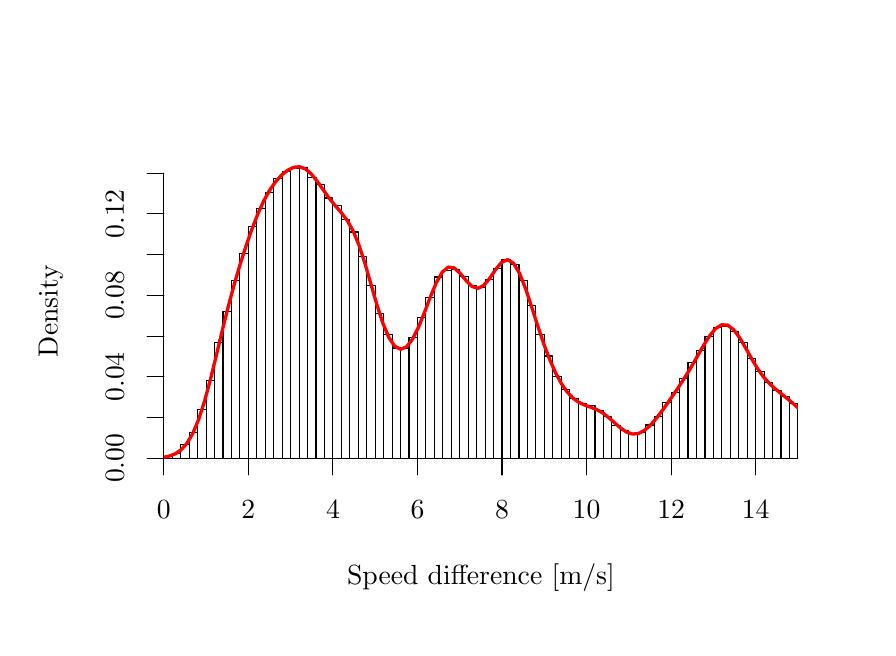
\begin{tikzpicture}[x=1pt,y=1pt]
\definecolor{fillColor}{RGB}{255,255,255}
\path[use as bounding box,fill=fillColor,fill opacity=0.00] (0,0) rectangle (303.53,216.81);
\begin{scope}
\path[clip] (  0.00,  0.00) rectangle (303.53,216.81);
\definecolor{drawColor}{RGB}{0,0,0}

\node[text=drawColor,anchor=base,inner sep=0pt, outer sep=0pt, scale=  1.00] at (163.77, 15.60) {Speed difference [m/s]};

\node[text=drawColor,rotate= 90.00,anchor=base,inner sep=0pt, outer sep=0pt, scale=  1.00] at ( 10.80,114.41) {Density};
\end{scope}
\begin{scope}
\path[clip] (  0.00,  0.00) rectangle (303.53,216.81);
\definecolor{drawColor}{RGB}{0,0,0}

\path[draw=drawColor,line width= 0.4pt,line join=round,line cap=round] ( 49.20, 61.20) -- (263.06, 61.20);

\path[draw=drawColor,line width= 0.4pt,line join=round,line cap=round] ( 49.20, 61.20) -- ( 49.20, 55.20);

\path[draw=drawColor,line width= 0.4pt,line join=round,line cap=round] ( 79.75, 61.20) -- ( 79.75, 55.20);

\path[draw=drawColor,line width= 0.4pt,line join=round,line cap=round] (110.30, 61.20) -- (110.30, 55.20);

\path[draw=drawColor,line width= 0.4pt,line join=round,line cap=round] (140.85, 61.20) -- (140.85, 55.20);

\path[draw=drawColor,line width= 0.4pt,line join=round,line cap=round] (171.40, 61.20) -- (171.40, 55.20);

\path[draw=drawColor,line width= 0.4pt,line join=round,line cap=round] (201.96, 61.20) -- (201.96, 55.20);

\path[draw=drawColor,line width= 0.4pt,line join=round,line cap=round] (232.51, 61.20) -- (232.51, 55.20);

\path[draw=drawColor,line width= 0.4pt,line join=round,line cap=round] (263.06, 61.20) -- (263.06, 55.20);

\node[text=drawColor,anchor=base,inner sep=0pt, outer sep=0pt, scale=  1.00] at ( 49.20, 39.60) {0};

\node[text=drawColor,anchor=base,inner sep=0pt, outer sep=0pt, scale=  1.00] at ( 79.75, 39.60) {2};

\node[text=drawColor,anchor=base,inner sep=0pt, outer sep=0pt, scale=  1.00] at (110.30, 39.60) {4};

\node[text=drawColor,anchor=base,inner sep=0pt, outer sep=0pt, scale=  1.00] at (140.85, 39.60) {6};

\node[text=drawColor,anchor=base,inner sep=0pt, outer sep=0pt, scale=  1.00] at (171.40, 39.60) {8};

\node[text=drawColor,anchor=base,inner sep=0pt, outer sep=0pt, scale=  1.00] at (201.96, 39.60) {10};

\node[text=drawColor,anchor=base,inner sep=0pt, outer sep=0pt, scale=  1.00] at (232.51, 39.60) {12};

\node[text=drawColor,anchor=base,inner sep=0pt, outer sep=0pt, scale=  1.00] at (263.06, 39.60) {14};

\path[draw=drawColor,line width= 0.4pt,line join=round,line cap=round] ( 49.20, 61.20) -- ( 49.20,164.23);

\path[draw=drawColor,line width= 0.4pt,line join=round,line cap=round] ( 49.20, 61.20) -- ( 43.20, 61.20);

\path[draw=drawColor,line width= 0.4pt,line join=round,line cap=round] ( 49.20, 75.92) -- ( 43.20, 75.92);

\path[draw=drawColor,line width= 0.4pt,line join=round,line cap=round] ( 49.20, 90.64) -- ( 43.20, 90.64);

\path[draw=drawColor,line width= 0.4pt,line join=round,line cap=round] ( 49.20,105.36) -- ( 43.20,105.36);

\path[draw=drawColor,line width= 0.4pt,line join=round,line cap=round] ( 49.20,120.07) -- ( 43.20,120.07);

\path[draw=drawColor,line width= 0.4pt,line join=round,line cap=round] ( 49.20,134.79) -- ( 43.20,134.79);

\path[draw=drawColor,line width= 0.4pt,line join=round,line cap=round] ( 49.20,149.51) -- ( 43.20,149.51);

\path[draw=drawColor,line width= 0.4pt,line join=round,line cap=round] ( 49.20,164.23) -- ( 43.20,164.23);

\node[text=drawColor,rotate= 90.00,anchor=base,inner sep=0pt, outer sep=0pt, scale=  1.00] at ( 34.80, 61.20) {0.00};

\node[text=drawColor,rotate= 90.00,anchor=base,inner sep=0pt, outer sep=0pt, scale=  1.00] at ( 34.80, 90.64) {0.04};

\node[text=drawColor,rotate= 90.00,anchor=base,inner sep=0pt, outer sep=0pt, scale=  1.00] at ( 34.80,120.07) {0.08};

\node[text=drawColor,rotate= 90.00,anchor=base,inner sep=0pt, outer sep=0pt, scale=  1.00] at ( 34.80,149.51) {0.12};
\end{scope}
\begin{scope}
\path[clip] ( 49.20, 61.20) rectangle (278.33,167.61);
\definecolor{drawColor}{RGB}{0,0,0}

\path[draw=drawColor,line width= 0.4pt,line join=round,line cap=round] ( -2.74, 61.20) rectangle (  0.32, 61.20);

\path[draw=drawColor,line width= 0.4pt,line join=round,line cap=round] (  0.32, 61.20) rectangle (  3.37, 61.20);

\path[draw=drawColor,line width= 0.4pt,line join=round,line cap=round] (  3.37, 61.20) rectangle (  6.43, 61.20);

\path[draw=drawColor,line width= 0.4pt,line join=round,line cap=round] (  6.43, 61.20) rectangle (  9.48, 61.20);

\path[draw=drawColor,line width= 0.4pt,line join=round,line cap=round] (  9.48, 61.20) rectangle ( 12.54, 61.20);

\path[draw=drawColor,line width= 0.4pt,line join=round,line cap=round] ( 12.54, 61.20) rectangle ( 15.59, 61.20);

\path[draw=drawColor,line width= 0.4pt,line join=round,line cap=round] ( 15.59, 61.20) rectangle ( 18.65, 61.20);

\path[draw=drawColor,line width= 0.4pt,line join=round,line cap=round] ( 18.65, 61.20) rectangle ( 21.70, 61.20);

\path[draw=drawColor,line width= 0.4pt,line join=round,line cap=round] ( 21.70, 61.20) rectangle ( 24.76, 61.20);

\path[draw=drawColor,line width= 0.4pt,line join=round,line cap=round] ( 24.76, 61.20) rectangle ( 27.81, 61.20);

\path[draw=drawColor,line width= 0.4pt,line join=round,line cap=round] ( 27.81, 61.20) rectangle ( 30.87, 61.20);

\path[draw=drawColor,line width= 0.4pt,line join=round,line cap=round] ( 30.87, 61.20) rectangle ( 33.92, 61.20);

\path[draw=drawColor,line width= 0.4pt,line join=round,line cap=round] ( 33.92, 61.20) rectangle ( 36.98, 61.20);

\path[draw=drawColor,line width= 0.4pt,line join=round,line cap=round] ( 36.98, 61.20) rectangle ( 40.03, 61.20);

\path[draw=drawColor,line width= 0.4pt,line join=round,line cap=round] ( 40.03, 61.20) rectangle ( 43.09, 61.22);

\path[draw=drawColor,line width= 0.4pt,line join=round,line cap=round] ( 43.09, 61.20) rectangle ( 46.14, 61.27);

\path[draw=drawColor,line width= 0.4pt,line join=round,line cap=round] ( 46.14, 61.20) rectangle ( 49.20, 61.42);

\path[draw=drawColor,line width= 0.4pt,line join=round,line cap=round] ( 49.20, 61.20) rectangle ( 52.26, 61.94);

\path[draw=drawColor,line width= 0.4pt,line join=round,line cap=round] ( 52.26, 61.20) rectangle ( 55.31, 63.05);

\path[draw=drawColor,line width= 0.4pt,line join=round,line cap=round] ( 55.31, 61.20) rectangle ( 58.37, 66.04);

\path[draw=drawColor,line width= 0.4pt,line join=round,line cap=round] ( 58.37, 61.20) rectangle ( 61.42, 70.58);

\path[draw=drawColor,line width= 0.4pt,line join=round,line cap=round] ( 61.42, 61.20) rectangle ( 64.48, 78.77);

\path[draw=drawColor,line width= 0.4pt,line join=round,line cap=round] ( 64.48, 61.20) rectangle ( 67.53, 89.26);

\path[draw=drawColor,line width= 0.4pt,line join=round,line cap=round] ( 67.53, 61.20) rectangle ( 70.59,103.07);

\path[draw=drawColor,line width= 0.4pt,line join=round,line cap=round] ( 70.59, 61.20) rectangle ( 73.64,114.13);

\path[draw=drawColor,line width= 0.4pt,line join=round,line cap=round] ( 73.64, 61.20) rectangle ( 76.70,125.48);

\path[draw=drawColor,line width= 0.4pt,line join=round,line cap=round] ( 76.70, 61.20) rectangle ( 79.75,135.26);

\path[draw=drawColor,line width= 0.4pt,line join=round,line cap=round] ( 79.75, 61.20) rectangle ( 82.81,145.00);

\path[draw=drawColor,line width= 0.4pt,line join=round,line cap=round] ( 82.81, 61.20) rectangle ( 85.86,151.37);

\path[draw=drawColor,line width= 0.4pt,line join=round,line cap=round] ( 85.86, 61.20) rectangle ( 88.92,157.32);

\path[draw=drawColor,line width= 0.4pt,line join=round,line cap=round] ( 88.92, 61.20) rectangle ( 91.97,162.35);

\path[draw=drawColor,line width= 0.4pt,line join=round,line cap=round] ( 91.97, 61.20) rectangle ( 95.03,164.90);

\path[draw=drawColor,line width= 0.4pt,line join=round,line cap=round] ( 95.03, 61.20) rectangle ( 98.08,165.90);

\path[draw=drawColor,line width= 0.4pt,line join=round,line cap=round] ( 98.08, 61.20) rectangle (101.14,166.42);

\path[draw=drawColor,line width= 0.4pt,line join=round,line cap=round] (101.14, 61.20) rectangle (104.19,162.61);

\path[draw=drawColor,line width= 0.4pt,line join=round,line cap=round] (104.19, 61.20) rectangle (107.25,160.24);

\path[draw=drawColor,line width= 0.4pt,line join=round,line cap=round] (107.25, 61.20) rectangle (110.30,155.25);

\path[draw=drawColor,line width= 0.4pt,line join=round,line cap=round] (110.30, 61.20) rectangle (113.36,152.41);

\path[draw=drawColor,line width= 0.4pt,line join=round,line cap=round] (113.36, 61.20) rectangle (116.41,147.47);

\path[draw=drawColor,line width= 0.4pt,line join=round,line cap=round] (116.41, 61.20) rectangle (119.47,142.96);

\path[draw=drawColor,line width= 0.4pt,line join=round,line cap=round] (119.47, 61.20) rectangle (122.52,134.19);

\path[draw=drawColor,line width= 0.4pt,line join=round,line cap=round] (122.52, 61.20) rectangle (125.58,123.50);

\path[draw=drawColor,line width= 0.4pt,line join=round,line cap=round] (125.58, 61.20) rectangle (128.63,113.59);

\path[draw=drawColor,line width= 0.4pt,line join=round,line cap=round] (128.63, 61.20) rectangle (131.69,106.09);

\path[draw=drawColor,line width= 0.4pt,line join=round,line cap=round] (131.69, 61.20) rectangle (134.74,101.04);

\path[draw=drawColor,line width= 0.4pt,line join=round,line cap=round] (134.74, 61.20) rectangle (137.80,101.03);

\path[draw=drawColor,line width= 0.4pt,line join=round,line cap=round] (137.80, 61.20) rectangle (140.85,104.93);

\path[draw=drawColor,line width= 0.4pt,line join=round,line cap=round] (140.85, 61.20) rectangle (143.91,112.07);

\path[draw=drawColor,line width= 0.4pt,line join=round,line cap=round] (143.91, 61.20) rectangle (146.96,119.40);

\path[draw=drawColor,line width= 0.4pt,line join=round,line cap=round] (146.96, 61.20) rectangle (150.02,126.70);

\path[draw=drawColor,line width= 0.4pt,line join=round,line cap=round] (150.02, 61.20) rectangle (153.07,129.22);

\path[draw=drawColor,line width= 0.4pt,line join=round,line cap=round] (153.07, 61.20) rectangle (156.13,129.40);

\path[draw=drawColor,line width= 0.4pt,line join=round,line cap=round] (156.13, 61.20) rectangle (159.18,126.86);

\path[draw=drawColor,line width= 0.4pt,line join=round,line cap=round] (159.18, 61.20) rectangle (162.24,123.78);

\path[draw=drawColor,line width= 0.4pt,line join=round,line cap=round] (162.24, 61.20) rectangle (165.29,122.78);

\path[draw=drawColor,line width= 0.4pt,line join=round,line cap=round] (165.29, 61.20) rectangle (168.35,125.73);

\path[draw=drawColor,line width= 0.4pt,line join=round,line cap=round] (168.35, 61.20) rectangle (171.40,129.85);

\path[draw=drawColor,line width= 0.4pt,line join=round,line cap=round] (171.40, 61.20) rectangle (174.46,133.00);

\path[draw=drawColor,line width= 0.4pt,line join=round,line cap=round] (174.46, 61.20) rectangle (177.52,131.07);

\path[draw=drawColor,line width= 0.4pt,line join=round,line cap=round] (177.52, 61.20) rectangle (180.57,125.42);

\path[draw=drawColor,line width= 0.4pt,line join=round,line cap=round] (180.57, 61.20) rectangle (183.63,116.34);

\path[draw=drawColor,line width= 0.4pt,line join=round,line cap=round] (183.63, 61.20) rectangle (186.68,106.08);

\path[draw=drawColor,line width= 0.4pt,line join=round,line cap=round] (186.68, 61.20) rectangle (189.74, 98.16);

\path[draw=drawColor,line width= 0.4pt,line join=round,line cap=round] (189.74, 61.20) rectangle (192.79, 90.66);

\path[draw=drawColor,line width= 0.4pt,line join=round,line cap=round] (192.79, 61.20) rectangle (195.85, 86.08);

\path[draw=drawColor,line width= 0.4pt,line join=round,line cap=round] (195.85, 61.20) rectangle (198.90, 82.84);

\path[draw=drawColor,line width= 0.4pt,line join=round,line cap=round] (198.90, 61.20) rectangle (201.96, 80.90);

\path[draw=drawColor,line width= 0.4pt,line join=round,line cap=round] (201.96, 61.20) rectangle (205.01, 80.42);

\path[draw=drawColor,line width= 0.4pt,line join=round,line cap=round] (205.01, 61.20) rectangle (208.07, 78.61);

\path[draw=drawColor,line width= 0.4pt,line join=round,line cap=round] (208.07, 61.20) rectangle (211.12, 76.43);

\path[draw=drawColor,line width= 0.4pt,line join=round,line cap=round] (211.12, 61.20) rectangle (214.18, 73.14);

\path[draw=drawColor,line width= 0.4pt,line join=round,line cap=round] (214.18, 61.20) rectangle (217.23, 71.11);

\path[draw=drawColor,line width= 0.4pt,line join=round,line cap=round] (217.23, 61.20) rectangle (220.29, 70.08);

\path[draw=drawColor,line width= 0.4pt,line join=round,line cap=round] (220.29, 61.20) rectangle (223.34, 70.56);

\path[draw=drawColor,line width= 0.4pt,line join=round,line cap=round] (223.34, 61.20) rectangle (226.40, 73.22);

\path[draw=drawColor,line width= 0.4pt,line join=round,line cap=round] (226.40, 61.20) rectangle (229.45, 76.40);

\path[draw=drawColor,line width= 0.4pt,line join=round,line cap=round] (229.45, 61.20) rectangle (232.51, 81.25);

\path[draw=drawColor,line width= 0.4pt,line join=round,line cap=round] (232.51, 61.20) rectangle (235.56, 85.11);

\path[draw=drawColor,line width= 0.4pt,line join=round,line cap=round] (235.56, 61.20) rectangle (238.62, 90.01);

\path[draw=drawColor,line width= 0.4pt,line join=round,line cap=round] (238.62, 61.20) rectangle (241.67, 95.91);

\path[draw=drawColor,line width= 0.4pt,line join=round,line cap=round] (241.67, 61.20) rectangle (244.73,100.18);

\path[draw=drawColor,line width= 0.4pt,line join=round,line cap=round] (244.73, 61.20) rectangle (247.78,105.13);

\path[draw=drawColor,line width= 0.4pt,line join=round,line cap=round] (247.78, 61.20) rectangle (250.84,108.35);

\path[draw=drawColor,line width= 0.4pt,line join=round,line cap=round] (250.84, 61.20) rectangle (253.89,108.91);

\path[draw=drawColor,line width= 0.4pt,line join=round,line cap=round] (253.89, 61.20) rectangle (256.95,106.87);

\path[draw=drawColor,line width= 0.4pt,line join=round,line cap=round] (256.95, 61.20) rectangle (260.00,102.92);

\path[draw=drawColor,line width= 0.4pt,line join=round,line cap=round] (260.00, 61.20) rectangle (263.06, 97.42);

\path[draw=drawColor,line width= 0.4pt,line join=round,line cap=round] (263.06, 61.20) rectangle (266.11, 92.63);

\path[draw=drawColor,line width= 0.4pt,line join=round,line cap=round] (266.11, 61.20) rectangle (269.17, 88.73);

\path[draw=drawColor,line width= 0.4pt,line join=round,line cap=round] (269.17, 61.20) rectangle (272.22, 85.73);

\path[draw=drawColor,line width= 0.4pt,line join=round,line cap=round] (272.22, 61.20) rectangle (275.28, 83.68);

\path[draw=drawColor,line width= 0.4pt,line join=round,line cap=round] (275.28, 61.20) rectangle (278.33, 81.01);

\path[draw=drawColor,line width= 0.4pt,line join=round,line cap=round] (278.33, 61.20) rectangle (281.39, 78.20);

\path[draw=drawColor,line width= 0.4pt,line join=round,line cap=round] (281.39, 61.20) rectangle (284.44, 75.10);

\path[draw=drawColor,line width= 0.4pt,line join=round,line cap=round] (284.44, 61.20) rectangle (287.50, 71.65);

\path[draw=drawColor,line width= 0.4pt,line join=round,line cap=round] (287.50, 61.20) rectangle (290.55, 68.97);

\path[draw=drawColor,line width= 0.4pt,line join=round,line cap=round] (290.55, 61.20) rectangle (293.61, 66.55);

\path[draw=drawColor,line width= 0.4pt,line join=round,line cap=round] (293.61, 61.20) rectangle (296.66, 64.95);

\path[draw=drawColor,line width= 0.4pt,line join=round,line cap=round] (296.66, 61.20) rectangle (299.72, 63.55);

\path[draw=drawColor,line width= 0.4pt,line join=round,line cap=round] (299.72, 61.20) rectangle (302.77, 62.46);

\path[draw=drawColor,line width= 0.4pt,line join=round,line cap=round] (302.77, 61.20) rectangle (305.83, 61.82);
\definecolor{drawColor}{RGB}{255,0,0}

\path[draw=drawColor,line width= 1.2pt,line join=round,line cap=round] (  0.00, 61.20) --
	(  1.66, 61.20) --
	(  3.80, 61.20) --
	(  5.95, 61.20) --
	(  8.10, 61.20) --
	( 10.24, 61.20) --
	( 12.39, 61.20) --
	( 14.54, 61.20) --
	( 16.69, 61.20) --
	( 18.83, 61.20) --
	( 20.98, 61.20) --
	( 23.13, 61.20) --
	( 25.27, 61.20) --
	( 27.42, 61.20) --
	( 29.57, 61.20) --
	( 31.72, 61.20) --
	( 33.86, 61.20) --
	( 36.01, 61.20) --
	( 38.16, 61.20) --
	( 40.30, 61.21) --
	( 42.45, 61.22) --
	( 44.60, 61.26) --
	( 46.75, 61.35) --
	( 48.89, 61.55) --
	( 51.04, 61.96) --
	( 53.19, 62.75) --
	( 55.33, 64.17) --
	( 57.48, 66.53) --
	( 59.63, 70.13) --
	( 61.78, 75.24) --
	( 63.92, 81.88) --
	( 66.07, 89.84) --
	( 68.22, 98.61) --
	( 70.36,107.57) --
	( 72.51,116.19) --
	( 74.66,124.15) --
	( 76.81,131.42) --
	( 78.95,138.10) --
	( 81.10,144.22) --
	( 83.25,149.71) --
	( 85.40,154.42) --
	( 87.54,158.26) --
	( 89.69,161.28) --
	( 91.84,163.61) --
	( 93.98,165.31) --
	( 96.13,166.35) --
	( 98.28,166.56) --
	(100.43,165.73) --
	(102.57,163.86) --
	(104.72,161.16) --
	(106.87,158.08) --
	(109.01,155.10) --
	(111.16,152.45) --
	(113.31,149.98) --
	(115.46,147.15) --
	(117.60,143.34) --
	(119.75,138.12) --
	(121.90,131.54) --
	(124.04,124.12) --
	(126.19,116.66) --
	(128.34,110.02) --
	(130.49,104.89) --
	(132.63,101.68) --
	(134.78,100.57) --
	(136.93,101.50) --
	(139.07,104.28) --
	(141.22,108.58) --
	(143.37,113.89) --
	(145.52,119.54) --
	(147.66,124.69) --
	(149.81,128.48) --
	(151.96,130.30) --
	(154.10,130.00) --
	(156.25,128.06) --
	(158.40,125.45) --
	(160.55,123.32) --
	(162.69,122.61) --
	(164.84,123.71) --
	(166.99,126.30) --
	(169.13,129.47) --
	(171.28,132.05) --
	(173.43,132.98) --
	(175.58,131.65) --
	(177.72,128.04) --
	(179.87,122.62) --
	(182.02,116.17) --
	(184.17,109.44) --
	(186.31,103.02) --
	(188.46, 97.28) --
	(190.61, 92.38) --
	(192.75, 88.35) --
	(194.90, 85.22) --
	(197.05, 82.93) --
	(199.20, 81.40) --
	(201.34, 80.41) --
	(203.49, 79.66) --
	(205.64, 78.80) --
	(207.78, 77.59) --
	(209.93, 75.94) --
	(212.08, 74.02) --
	(214.23, 72.14) --
	(216.37, 70.69) --
	(218.52, 69.97) --
	(220.67, 70.14) --
	(222.81, 71.23) --
	(224.96, 73.10) --
	(227.11, 75.56) --
	(229.26, 78.39) --
	(231.40, 81.40) --
	(233.55, 84.50) --
	(235.70, 87.68) --
	(237.84, 91.02) --
	(239.99, 94.58) --
	(242.14, 98.34) --
	(244.29,102.09) --
	(246.43,105.48) --
	(248.58,108.07) --
	(250.73,109.44) --
	(252.87,109.35) --
	(255.02,107.76) --
	(257.17,104.92) --
	(259.32,101.28) --
	(261.46, 97.42) --
	(263.61, 93.82) --
	(265.76, 90.78) --
	(267.90, 88.34) --
	(270.05, 86.36) --
	(272.20, 84.61) --
	(274.35, 82.89) --
	(276.49, 81.08) --
	(278.64, 79.12) --
	(280.79, 77.04) --
	(282.94, 74.90) --
	(285.08, 72.77) --
	(287.23, 70.74) --
	(289.38, 68.87) --
	(291.52, 67.20) --
	(293.67, 65.76) --
	(295.82, 64.55) --
	(297.97, 63.59) --
	(300.11, 62.84) --
	(302.26, 62.29) --
	(303.53, 62.05);
\end{scope}
\end{tikzpicture}

	}
	\caption{The histogram shows the result of the conditional sampling according to \cref{alg:constrained simple}. The red line represents the true \ac{pdf}.}
	\label{fig:constrained simple}
\end{figure}

\begin{figure}
	\centering
	\resizebox{\columnwidth}{!}{%
		% Created by tikzDevice version 0.12.3 on 2021-02-01 12:22:52
% !TEX encoding = UTF-8 Unicode
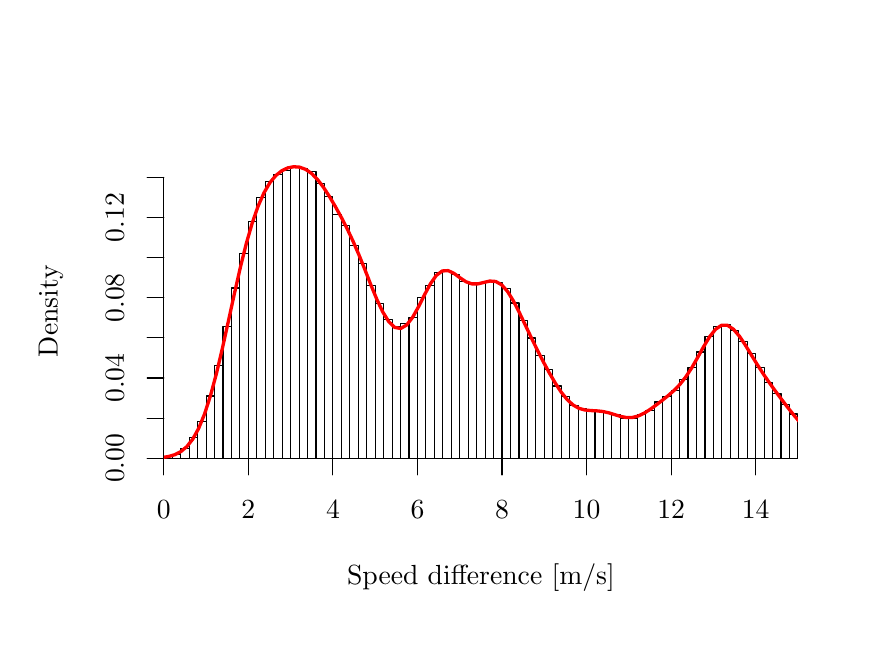
\begin{tikzpicture}[x=1pt,y=1pt]
\definecolor{fillColor}{RGB}{255,255,255}
\path[use as bounding box,fill=fillColor,fill opacity=0.00] (0,0) rectangle (303.53,216.81);
\begin{scope}
\path[clip] (  0.00,  0.00) rectangle (303.53,216.81);
\definecolor{drawColor}{RGB}{0,0,0}

\node[text=drawColor,anchor=base,inner sep=0pt, outer sep=0pt, scale=  1.00] at (163.77, 15.60) {Speed difference [m/s]};

\node[text=drawColor,rotate= 90.00,anchor=base,inner sep=0pt, outer sep=0pt, scale=  1.00] at ( 10.80,114.41) {Density};
\end{scope}
\begin{scope}
\path[clip] (  0.00,  0.00) rectangle (303.53,216.81);
\definecolor{drawColor}{RGB}{0,0,0}

\path[draw=drawColor,line width= 0.4pt,line join=round,line cap=round] ( 49.20, 61.20) -- (263.06, 61.20);

\path[draw=drawColor,line width= 0.4pt,line join=round,line cap=round] ( 49.20, 61.20) -- ( 49.20, 55.20);

\path[draw=drawColor,line width= 0.4pt,line join=round,line cap=round] ( 79.75, 61.20) -- ( 79.75, 55.20);

\path[draw=drawColor,line width= 0.4pt,line join=round,line cap=round] (110.30, 61.20) -- (110.30, 55.20);

\path[draw=drawColor,line width= 0.4pt,line join=round,line cap=round] (140.85, 61.20) -- (140.85, 55.20);

\path[draw=drawColor,line width= 0.4pt,line join=round,line cap=round] (171.40, 61.20) -- (171.40, 55.20);

\path[draw=drawColor,line width= 0.4pt,line join=round,line cap=round] (201.96, 61.20) -- (201.96, 55.20);

\path[draw=drawColor,line width= 0.4pt,line join=round,line cap=round] (232.51, 61.20) -- (232.51, 55.20);

\path[draw=drawColor,line width= 0.4pt,line join=round,line cap=round] (263.06, 61.20) -- (263.06, 55.20);

\node[text=drawColor,anchor=base,inner sep=0pt, outer sep=0pt, scale=  1.00] at ( 49.20, 39.60) {0};

\node[text=drawColor,anchor=base,inner sep=0pt, outer sep=0pt, scale=  1.00] at ( 79.75, 39.60) {2};

\node[text=drawColor,anchor=base,inner sep=0pt, outer sep=0pt, scale=  1.00] at (110.30, 39.60) {4};

\node[text=drawColor,anchor=base,inner sep=0pt, outer sep=0pt, scale=  1.00] at (140.85, 39.60) {6};

\node[text=drawColor,anchor=base,inner sep=0pt, outer sep=0pt, scale=  1.00] at (171.40, 39.60) {8};

\node[text=drawColor,anchor=base,inner sep=0pt, outer sep=0pt, scale=  1.00] at (201.96, 39.60) {10};

\node[text=drawColor,anchor=base,inner sep=0pt, outer sep=0pt, scale=  1.00] at (232.51, 39.60) {12};

\node[text=drawColor,anchor=base,inner sep=0pt, outer sep=0pt, scale=  1.00] at (263.06, 39.60) {14};

\path[draw=drawColor,line width= 0.4pt,line join=round,line cap=round] ( 49.20, 61.20) -- ( 49.20,162.69);

\path[draw=drawColor,line width= 0.4pt,line join=round,line cap=round] ( 49.20, 61.20) -- ( 43.20, 61.20);

\path[draw=drawColor,line width= 0.4pt,line join=round,line cap=round] ( 49.20, 75.70) -- ( 43.20, 75.70);

\path[draw=drawColor,line width= 0.4pt,line join=round,line cap=round] ( 49.20, 90.20) -- ( 43.20, 90.20);

\path[draw=drawColor,line width= 0.4pt,line join=round,line cap=round] ( 49.20,104.70) -- ( 43.20,104.70);

\path[draw=drawColor,line width= 0.4pt,line join=round,line cap=round] ( 49.20,119.19) -- ( 43.20,119.19);

\path[draw=drawColor,line width= 0.4pt,line join=round,line cap=round] ( 49.20,133.69) -- ( 43.20,133.69);

\path[draw=drawColor,line width= 0.4pt,line join=round,line cap=round] ( 49.20,148.19) -- ( 43.20,148.19);

\path[draw=drawColor,line width= 0.4pt,line join=round,line cap=round] ( 49.20,162.69) -- ( 43.20,162.69);

\node[text=drawColor,rotate= 90.00,anchor=base,inner sep=0pt, outer sep=0pt, scale=  1.00] at ( 34.80, 61.20) {0.00};

\node[text=drawColor,rotate= 90.00,anchor=base,inner sep=0pt, outer sep=0pt, scale=  1.00] at ( 34.80, 90.20) {0.04};

\node[text=drawColor,rotate= 90.00,anchor=base,inner sep=0pt, outer sep=0pt, scale=  1.00] at ( 34.80,119.19) {0.08};

\node[text=drawColor,rotate= 90.00,anchor=base,inner sep=0pt, outer sep=0pt, scale=  1.00] at ( 34.80,148.19) {0.12};
\end{scope}
\begin{scope}
\path[clip] ( 49.20, 61.20) rectangle (278.33,167.61);
\definecolor{drawColor}{RGB}{0,0,0}

\path[draw=drawColor,line width= 0.4pt,line join=round,line cap=round] ( -2.74, 61.20) rectangle (  0.32, 61.20);

\path[draw=drawColor,line width= 0.4pt,line join=round,line cap=round] (  0.32, 61.20) rectangle (  3.37, 61.20);

\path[draw=drawColor,line width= 0.4pt,line join=round,line cap=round] (  3.37, 61.20) rectangle (  6.43, 61.20);

\path[draw=drawColor,line width= 0.4pt,line join=round,line cap=round] (  6.43, 61.20) rectangle (  9.48, 61.20);

\path[draw=drawColor,line width= 0.4pt,line join=round,line cap=round] (  9.48, 61.20) rectangle ( 12.54, 61.20);

\path[draw=drawColor,line width= 0.4pt,line join=round,line cap=round] ( 12.54, 61.20) rectangle ( 15.59, 61.20);

\path[draw=drawColor,line width= 0.4pt,line join=round,line cap=round] ( 15.59, 61.20) rectangle ( 18.65, 61.20);

\path[draw=drawColor,line width= 0.4pt,line join=round,line cap=round] ( 18.65, 61.20) rectangle ( 21.70, 61.20);

\path[draw=drawColor,line width= 0.4pt,line join=round,line cap=round] ( 21.70, 61.20) rectangle ( 24.76, 61.20);

\path[draw=drawColor,line width= 0.4pt,line join=round,line cap=round] ( 24.76, 61.20) rectangle ( 27.81, 61.20);

\path[draw=drawColor,line width= 0.4pt,line join=round,line cap=round] ( 27.81, 61.20) rectangle ( 30.87, 61.20);

\path[draw=drawColor,line width= 0.4pt,line join=round,line cap=round] ( 30.87, 61.20) rectangle ( 33.92, 61.20);

\path[draw=drawColor,line width= 0.4pt,line join=round,line cap=round] ( 33.92, 61.20) rectangle ( 36.98, 61.20);

\path[draw=drawColor,line width= 0.4pt,line join=round,line cap=round] ( 36.98, 61.20) rectangle ( 40.03, 61.20);

\path[draw=drawColor,line width= 0.4pt,line join=round,line cap=round] ( 40.03, 61.20) rectangle ( 43.09, 61.21);

\path[draw=drawColor,line width= 0.4pt,line join=round,line cap=round] ( 43.09, 61.20) rectangle ( 46.14, 61.27);

\path[draw=drawColor,line width= 0.4pt,line join=round,line cap=round] ( 46.14, 61.20) rectangle ( 49.20, 61.46);

\path[draw=drawColor,line width= 0.4pt,line join=round,line cap=round] ( 49.20, 61.20) rectangle ( 52.26, 61.83);

\path[draw=drawColor,line width= 0.4pt,line join=round,line cap=round] ( 52.26, 61.20) rectangle ( 55.31, 62.73);

\path[draw=drawColor,line width= 0.4pt,line join=round,line cap=round] ( 55.31, 61.20) rectangle ( 58.37, 64.70);

\path[draw=drawColor,line width= 0.4pt,line join=round,line cap=round] ( 58.37, 61.20) rectangle ( 61.42, 68.79);

\path[draw=drawColor,line width= 0.4pt,line join=round,line cap=round] ( 61.42, 61.20) rectangle ( 64.48, 74.61);

\path[draw=drawColor,line width= 0.4pt,line join=round,line cap=round] ( 64.48, 61.20) rectangle ( 67.53, 83.73);

\path[draw=drawColor,line width= 0.4pt,line join=round,line cap=round] ( 67.53, 61.20) rectangle ( 70.59, 94.80);

\path[draw=drawColor,line width= 0.4pt,line join=round,line cap=round] ( 70.59, 61.20) rectangle ( 73.64,108.87);

\path[draw=drawColor,line width= 0.4pt,line join=round,line cap=round] ( 73.64, 61.20) rectangle ( 76.70,122.74);

\path[draw=drawColor,line width= 0.4pt,line join=round,line cap=round] ( 76.70, 61.20) rectangle ( 79.75,135.21);

\path[draw=drawColor,line width= 0.4pt,line join=round,line cap=round] ( 79.75, 61.20) rectangle ( 82.81,146.85);

\path[draw=drawColor,line width= 0.4pt,line join=round,line cap=round] ( 82.81, 61.20) rectangle ( 85.86,155.48);

\path[draw=drawColor,line width= 0.4pt,line join=round,line cap=round] ( 85.86, 61.20) rectangle ( 88.92,161.34);

\path[draw=drawColor,line width= 0.4pt,line join=round,line cap=round] ( 88.92, 61.20) rectangle ( 91.97,163.85);

\path[draw=drawColor,line width= 0.4pt,line join=round,line cap=round] ( 91.97, 61.20) rectangle ( 95.03,165.21);

\path[draw=drawColor,line width= 0.4pt,line join=round,line cap=round] ( 95.03, 61.20) rectangle ( 98.08,166.24);

\path[draw=drawColor,line width= 0.4pt,line join=round,line cap=round] ( 98.08, 61.20) rectangle (101.14,165.85);

\path[draw=drawColor,line width= 0.4pt,line join=round,line cap=round] (101.14, 61.20) rectangle (104.19,164.74);

\path[draw=drawColor,line width= 0.4pt,line join=round,line cap=round] (104.19, 61.20) rectangle (107.25,160.42);

\path[draw=drawColor,line width= 0.4pt,line join=round,line cap=round] (107.25, 61.20) rectangle (110.30,155.81);

\path[draw=drawColor,line width= 0.4pt,line join=round,line cap=round] (110.30, 61.20) rectangle (113.36,149.35);

\path[draw=drawColor,line width= 0.4pt,line join=round,line cap=round] (113.36, 61.20) rectangle (116.41,145.23);

\path[draw=drawColor,line width= 0.4pt,line join=round,line cap=round] (116.41, 61.20) rectangle (119.47,137.98);

\path[draw=drawColor,line width= 0.4pt,line join=round,line cap=round] (119.47, 61.20) rectangle (122.52,131.73);

\path[draw=drawColor,line width= 0.4pt,line join=round,line cap=round] (122.52, 61.20) rectangle (125.58,123.54);

\path[draw=drawColor,line width= 0.4pt,line join=round,line cap=round] (125.58, 61.20) rectangle (128.63,117.26);

\path[draw=drawColor,line width= 0.4pt,line join=round,line cap=round] (128.63, 61.20) rectangle (131.69,111.30);

\path[draw=drawColor,line width= 0.4pt,line join=round,line cap=round] (131.69, 61.20) rectangle (134.74,108.69);

\path[draw=drawColor,line width= 0.4pt,line join=round,line cap=round] (134.74, 61.20) rectangle (137.80,109.98);

\path[draw=drawColor,line width= 0.4pt,line join=round,line cap=round] (137.80, 61.20) rectangle (140.85,112.01);

\path[draw=drawColor,line width= 0.4pt,line join=round,line cap=round] (140.85, 61.20) rectangle (143.91,119.27);

\path[draw=drawColor,line width= 0.4pt,line join=round,line cap=round] (143.91, 61.20) rectangle (146.96,123.61);

\path[draw=drawColor,line width= 0.4pt,line join=round,line cap=round] (146.96, 61.20) rectangle (150.02,128.48);

\path[draw=drawColor,line width= 0.4pt,line join=round,line cap=round] (150.02, 61.20) rectangle (153.07,128.65);

\path[draw=drawColor,line width= 0.4pt,line join=round,line cap=round] (153.07, 61.20) rectangle (156.13,127.60);

\path[draw=drawColor,line width= 0.4pt,line join=round,line cap=round] (156.13, 61.20) rectangle (159.18,125.14);

\path[draw=drawColor,line width= 0.4pt,line join=round,line cap=round] (159.18, 61.20) rectangle (162.24,124.11);

\path[draw=drawColor,line width= 0.4pt,line join=round,line cap=round] (162.24, 61.20) rectangle (165.29,124.22);

\path[draw=drawColor,line width= 0.4pt,line join=round,line cap=round] (165.29, 61.20) rectangle (168.35,125.20);

\path[draw=drawColor,line width= 0.4pt,line join=round,line cap=round] (168.35, 61.20) rectangle (171.40,124.60);

\path[draw=drawColor,line width= 0.4pt,line join=round,line cap=round] (171.40, 61.20) rectangle (174.46,122.71);

\path[draw=drawColor,line width= 0.4pt,line join=round,line cap=round] (174.46, 61.20) rectangle (177.52,117.32);

\path[draw=drawColor,line width= 0.4pt,line join=round,line cap=round] (177.52, 61.20) rectangle (180.57,110.99);

\path[draw=drawColor,line width= 0.4pt,line join=round,line cap=round] (180.57, 61.20) rectangle (183.63,104.66);

\path[draw=drawColor,line width= 0.4pt,line join=round,line cap=round] (183.63, 61.20) rectangle (186.68, 98.49);

\path[draw=drawColor,line width= 0.4pt,line join=round,line cap=round] (186.68, 61.20) rectangle (189.74, 93.24);

\path[draw=drawColor,line width= 0.4pt,line join=round,line cap=round] (189.74, 61.20) rectangle (192.79, 87.34);

\path[draw=drawColor,line width= 0.4pt,line join=round,line cap=round] (192.79, 61.20) rectangle (195.85, 83.47);

\path[draw=drawColor,line width= 0.4pt,line join=round,line cap=round] (195.85, 61.20) rectangle (198.90, 80.19);

\path[draw=drawColor,line width= 0.4pt,line join=round,line cap=round] (198.90, 61.20) rectangle (201.96, 79.05);

\path[draw=drawColor,line width= 0.4pt,line join=round,line cap=round] (201.96, 61.20) rectangle (205.01, 78.20);

\path[draw=drawColor,line width= 0.4pt,line join=round,line cap=round] (205.01, 61.20) rectangle (208.07, 78.55);

\path[draw=drawColor,line width= 0.4pt,line join=round,line cap=round] (208.07, 61.20) rectangle (211.12, 77.69);

\path[draw=drawColor,line width= 0.4pt,line join=round,line cap=round] (211.12, 61.20) rectangle (214.18, 76.92);

\path[draw=drawColor,line width= 0.4pt,line join=round,line cap=round] (214.18, 61.20) rectangle (217.23, 75.71);

\path[draw=drawColor,line width= 0.4pt,line join=round,line cap=round] (217.23, 61.20) rectangle (220.29, 75.74);

\path[draw=drawColor,line width= 0.4pt,line join=round,line cap=round] (220.29, 61.20) rectangle (223.34, 77.04);

\path[draw=drawColor,line width= 0.4pt,line join=round,line cap=round] (223.34, 61.20) rectangle (226.40, 78.57);

\path[draw=drawColor,line width= 0.4pt,line join=round,line cap=round] (226.40, 61.20) rectangle (229.45, 81.55);

\path[draw=drawColor,line width= 0.4pt,line join=round,line cap=round] (229.45, 61.20) rectangle (232.51, 83.64);

\path[draw=drawColor,line width= 0.4pt,line join=round,line cap=round] (232.51, 61.20) rectangle (235.56, 85.85);

\path[draw=drawColor,line width= 0.4pt,line join=round,line cap=round] (235.56, 61.20) rectangle (238.62, 89.66);

\path[draw=drawColor,line width= 0.4pt,line join=round,line cap=round] (238.62, 61.20) rectangle (241.67, 94.17);

\path[draw=drawColor,line width= 0.4pt,line join=round,line cap=round] (241.67, 61.20) rectangle (244.73, 99.62);

\path[draw=drawColor,line width= 0.4pt,line join=round,line cap=round] (244.73, 61.20) rectangle (247.78,105.33);

\path[draw=drawColor,line width= 0.4pt,line join=round,line cap=round] (247.78, 61.20) rectangle (250.84,108.83);

\path[draw=drawColor,line width= 0.4pt,line join=round,line cap=round] (250.84, 61.20) rectangle (253.89,109.39);

\path[draw=drawColor,line width= 0.4pt,line join=round,line cap=round] (253.89, 61.20) rectangle (256.95,107.23);

\path[draw=drawColor,line width= 0.4pt,line join=round,line cap=round] (256.95, 61.20) rectangle (260.00,103.29);

\path[draw=drawColor,line width= 0.4pt,line join=round,line cap=round] (260.00, 61.20) rectangle (263.06, 98.91);

\path[draw=drawColor,line width= 0.4pt,line join=round,line cap=round] (263.06, 61.20) rectangle (266.11, 93.99);

\path[draw=drawColor,line width= 0.4pt,line join=round,line cap=round] (266.11, 61.20) rectangle (269.17, 88.44);

\path[draw=drawColor,line width= 0.4pt,line join=round,line cap=round] (269.17, 61.20) rectangle (272.22, 84.54);

\path[draw=drawColor,line width= 0.4pt,line join=round,line cap=round] (272.22, 61.20) rectangle (275.28, 80.69);

\path[draw=drawColor,line width= 0.4pt,line join=round,line cap=round] (275.28, 61.20) rectangle (278.33, 77.20);

\path[draw=drawColor,line width= 0.4pt,line join=round,line cap=round] (278.33, 61.20) rectangle (281.39, 73.09);

\path[draw=drawColor,line width= 0.4pt,line join=round,line cap=round] (281.39, 61.20) rectangle (284.44, 70.50);

\path[draw=drawColor,line width= 0.4pt,line join=round,line cap=round] (284.44, 61.20) rectangle (287.50, 67.88);

\path[draw=drawColor,line width= 0.4pt,line join=round,line cap=round] (287.50, 61.20) rectangle (290.55, 66.40);

\path[draw=drawColor,line width= 0.4pt,line join=round,line cap=round] (290.55, 61.20) rectangle (293.61, 64.88);

\path[draw=drawColor,line width= 0.4pt,line join=round,line cap=round] (293.61, 61.20) rectangle (296.66, 63.91);

\path[draw=drawColor,line width= 0.4pt,line join=round,line cap=round] (296.66, 61.20) rectangle (299.72, 63.11);

\path[draw=drawColor,line width= 0.4pt,line join=round,line cap=round] (299.72, 61.20) rectangle (302.77, 62.45);

\path[draw=drawColor,line width= 0.4pt,line join=round,line cap=round] (302.77, 61.20) rectangle (305.83, 62.05);
\definecolor{drawColor}{RGB}{255,0,0}

\path[draw=drawColor,line width= 1.2pt,line join=round,line cap=round] (  0.00, 61.20) --
	(  1.66, 61.20) --
	(  3.80, 61.20) --
	(  5.95, 61.20) --
	(  8.10, 61.20) --
	( 10.24, 61.20) --
	( 12.39, 61.20) --
	( 14.54, 61.20) --
	( 16.69, 61.20) --
	( 18.83, 61.20) --
	( 20.98, 61.20) --
	( 23.13, 61.20) --
	( 25.27, 61.20) --
	( 27.42, 61.20) --
	( 29.57, 61.20) --
	( 31.72, 61.20) --
	( 33.86, 61.20) --
	( 36.01, 61.20) --
	( 38.16, 61.20) --
	( 40.30, 61.21) --
	( 42.45, 61.23) --
	( 44.60, 61.26) --
	( 46.75, 61.35) --
	( 48.89, 61.53) --
	( 51.04, 61.88) --
	( 53.19, 62.52) --
	( 55.33, 63.62) --
	( 57.48, 65.40) --
	( 59.63, 68.11) --
	( 61.78, 71.99) --
	( 63.92, 77.22) --
	( 66.07, 83.88) --
	( 68.22, 91.88) --
	( 70.36,100.95) --
	( 72.51,110.68) --
	( 74.66,120.53) --
	( 76.81,129.99) --
	( 78.95,138.62) --
	( 81.10,146.10) --
	( 83.25,152.29) --
	( 85.40,157.16) --
	( 87.54,160.81) --
	( 89.69,163.40) --
	( 91.84,165.12) --
	( 93.98,166.14) --
	( 96.13,166.56) --
	( 98.28,166.40) --
	(100.43,165.62) --
	(102.57,164.15) --
	(104.72,161.96) --
	(106.87,159.14) --
	(109.01,155.84) --
	(111.16,152.20) --
	(113.31,148.31) --
	(115.46,144.13) --
	(117.60,139.58) --
	(119.75,134.60) --
	(121.90,129.27) --
	(124.04,123.80) --
	(126.19,118.58) --
	(128.34,114.03) --
	(130.49,110.56) --
	(132.63,108.51) --
	(134.78,108.10) --
	(136.93,109.35) --
	(139.07,112.10) --
	(141.22,115.94) --
	(143.37,120.24) --
	(145.52,124.25) --
	(147.66,127.29) --
	(149.81,128.90) --
	(151.96,129.02) --
	(154.10,127.98) --
	(156.25,126.41) --
	(158.40,124.99) --
	(160.55,124.22) --
	(162.69,124.23) --
	(164.84,124.75) --
	(166.99,125.25) --
	(169.13,125.10) --
	(171.28,123.89) --
	(173.43,121.45) --
	(175.58,117.95) --
	(177.72,113.74) --
	(179.87,109.23) --
	(182.02,104.70) --
	(184.17,100.31) --
	(186.31, 96.11) --
	(188.46, 92.13) --
	(190.61, 88.44) --
	(192.75, 85.16) --
	(194.90, 82.47) --
	(197.05, 80.49) --
	(199.20, 79.26) --
	(201.34, 78.66) --
	(203.49, 78.45) --
	(205.64, 78.35) --
	(207.78, 78.12) --
	(209.93, 77.65) --
	(212.08, 76.99) --
	(214.23, 76.34) --
	(216.37, 75.93) --
	(218.52, 75.96) --
	(220.67, 76.51) --
	(222.81, 77.53) --
	(224.96, 78.90) --
	(227.11, 80.46) --
	(229.26, 82.11) --
	(231.40, 83.82) --
	(233.55, 85.70) --
	(235.70, 87.92) --
	(237.84, 90.65) --
	(239.99, 93.96) --
	(242.14, 97.71) --
	(244.29,101.60) --
	(246.43,105.14) --
	(248.58,107.84) --
	(250.73,109.27) --
	(252.87,109.26) --
	(255.02,107.85) --
	(257.17,105.33) --
	(259.32,102.11) --
	(261.46, 98.60) --
	(263.61, 95.11) --
	(265.76, 91.78) --
	(267.90, 88.65) --
	(270.05, 85.67) --
	(272.20, 82.78) --
	(274.35, 79.96) --
	(276.49, 77.24) --
	(278.64, 74.70) --
	(280.79, 72.40) --
	(282.94, 70.40) --
	(285.08, 68.70) --
	(287.23, 67.30) --
	(289.38, 66.15) --
	(291.52, 65.20) --
	(293.67, 64.42) --
	(295.82, 63.76) --
	(297.97, 63.20) --
	(300.11, 62.72) --
	(302.26, 62.32) --
	(303.53, 62.12);
\end{scope}
\end{tikzpicture}

	}
	\caption{The histogram shows the result of the conditional sampling according to \cref{alg:constrained hard}. The red line represents the true \ac{pdf}.}
	\label{fig:constrained hard}
\end{figure}
